\documentclass[11pt]{article}

%\usepackage[backend=biber]{biblatex}
%\addbibresource{references.bib}

%\usepackage[margin=1in]{geometry}
\usepackage{amsfonts, amsmath, amssymb, mathtools} % --> to typeset math
\usepackage{wrapfig}
\newcommand{\iu}{{i\mkern1mu}}
\DeclareMathOperator{\arccot}{arccot}
\DeclareMathOperator{\argsinh}{argsinh}
\DeclareMathOperator{\argcosh}{argcosh}
\DeclareMathOperator{\argtanh}{argtanh}
\DeclareMathOperator{\argcoth}{argcoth}
\DeclareMathOperator{\sgn}{sgn}
\newcommand{\floor}[1]{\left\lfloor #1 \right\rfloor}
\newcommand{\ceil}[1]{\left\lceil #1 \right\rceil}
\DeclareMathOperator{\tr}{Tr}
\DeclareMathOperator*{\argmax}{arg\,max}
\DeclareMathOperator*{\argmin}{arg\,min}

\usepackage{accents}
\newcommand{\ut}[1]{\underaccent{\tilde}{#1}}
\renewcommand{\vec}[1]{\ut{#1}}

\usepackage{cancel}

\usepackage{multicol}
\usepackage{hhline}
\usepackage[shortlabels]{enumitem}

\usepackage{caption}
\usepackage{placeins}
\usepackage{graphicx}
\usepackage{pdfpages}
\usepackage{subcaption}
\usepackage{fancyhdr}
\usepackage{float}
\usepackage{geometry}
\setlength{\textheight}{22.5cm}
\usepackage{indentfirst}
\usepackage{array}
\usepackage{tabularx}
\usepackage{booktabs}
\usepackage{longtable}
\usepackage[siunitx, straightvoltages]{circuitikz}
\usetikzlibrary{shapes.geometric, arrows, arrows.meta, shapes.misc}
\usetikzlibrary{calc}
\usepackage{xcolor}
\usepackage{pgfgantt}
\usepackage{hyperref}
\usepackage{bm}
\usepackage{background}
% svg must load before babelbib: both define \test@number (svg via scrbase
% with \newcommand, babelbib with \providecommand), so svg has to come first.
\usepackage{svg}
\usepackage[fixlanguage]{babelbib}
\usepackage[english]{babel}
\usepackage[authoryear]{natbib}

% --- Images live in the images/ subfolder (Overleaf parent = Report) ---
\graphicspath{{images/}}
% --- Vector diagrams are included directly as SVG via \includesvg (svg
% package, loaded above). Needs Inkscape + shell-escape; Overleaf enables
% both automatically. ---
\svgpath{{images/}}
% Let Inkscape render the SVG text into the PDF instead of extracting it as a
% LaTeX overlay: the diagrams contain code identifiers with underscores
% (LEFT_WHEEL, to_motor, link_up, ...) that LaTeX would read as math subscripts.
\svgsetup{inkscapelatex=false}

% --- Wrapping table column types ---
\newcolumntype{Y}{>{\raggedright\arraybackslash}X}
\newcolumntype{P}[1]{>{\raggedright\arraybackslash}p{#1}}
\renewcommand{\arraystretch}{1.15}
\setlength{\LTleft}{0pt}
\setlength{\LTright}{0pt}

% --- Colours for the two placeholder kinds ---
\definecolor{phimage}{RGB}{180,83,9}    % IMAGE = external photo/screenshot
\definecolor{phdiagram}{RGB}{79,70,229}  % DIAGRAM = our generated vector figure

% --- IMAGE helper: an EXTERNAL photo or screenshot (not one of our diagrams).
% Renders the file if present, else a labelled IMAGE placeholder. ---
% #1 = filename (in images/), #2 = width fraction, #3 = caption, #4 = label
\newcommand{\reportfig}[4]{%
\begin{figure}[H]
    \centering
    \IfFileExists{images/#1}{%
        \includegraphics[width=#2\linewidth]{#1}%
    }{%
        \fcolorbox{phimage}{phimage!6}{\parbox[c][0.24\textheight][c]{0.88\linewidth}{\centering
        {\sffamily\bfseries\color{phimage}[IMAGE]} {\itshape external photo or screenshot}\\[2pt]
        {\itshape add the file \texttt{images/#1}}\\[6pt]\normalfont #3}}%
    }
    \caption{#3}\label{#4}
\end{figure}}

% --- DIAGRAM (vector figure) helper: one of OUR generated diagrams (from
% diagrams.html / diagram_svgs/). Prefer a vector PDF (converted from the SVG),
% fall back to a PNG screenshot, else a labelled DIAGRAM placeholder. ---
% #1 = basename (no extension), #2 = width fraction, #3 = caption, #4 = label
\newcommand{\vecfig}[4]{%
\begin{figure}[H]
    \centering
    \IfFileExists{images/#1.svg}{%
        \includesvg[width=#2\linewidth]{#1}%
    }{\IfFileExists{images/#1.pdf}{%
        \includegraphics[width=#2\linewidth]{#1.pdf}%
    }{\IfFileExists{images/#1.png}{%
        \includegraphics[width=#2\linewidth]{#1.png}%
    }{%
        \fcolorbox{phdiagram}{phdiagram!6}{\parbox[c][0.24\textheight][c]{0.88\linewidth}{\centering
        {\sffamily\bfseries\color{phdiagram}[DIAGRAM]} {\itshape our vector figure}\\[2pt]
        {\itshape add \texttt{images/#1.svg}}\\[6pt]\normalfont #3}}%
    }}}
    \caption{#3}\label{#4}
\end{figure}}

% --- Gantt colours ---
\definecolor{barblue}{RGB}{153,204,254}
\definecolor{groupblue}{RGB}{51,102,254}
\definecolor{linkred}{RGB}{165,0,33}

\makeatletter
\def\bg@material{%
\begin{tikzpicture}[remember picture,overlay]
\node [rotate=0,scale=0.5,opacity=0.2,color=blue!30,xshift=-5mm,yshift=10mm]
at (current page.south east)  [anchor=south east]{\IfFileExists{images/LogoEPFL.png}{\includegraphics[height=.06\paperheight]{LogoEPFL.png}}{}};
\end{tikzpicture}}
\makeatother

\newcommand\tab[1][0.7cm]{\hspace*{#1}}

\fancypagestyle{plain}{}
\pagestyle{fancy}
\fancyhead{}
\fancyfoot{}
\fancyfoot[C]{\thepage}
\fancyhead[L]{Robotics Competition}
\fancyhead[C]{Team 6 - Eye Robot}
\fancyhead[R]{Spring 2026}
\renewcommand{\headrulewidth}{0.4pt}

\setlength{\footskip}{30pt}
\pagenumbering{roman}

\begin{document}

\begin{titlepage}
\begin{center}
\Huge{\textbf{Interdisciplinary Robotic Competition}} \\[1cm]
\Huge{\textbf{Team 6 - Eye Robot}} \\[1cm]
\Large{\textbf{\textit{\textbf{Pedro Conde Salvarelli}}}} \\
\Large{\textbf{\textit{Nathan Kack Kack}}} \\
\Large{\textbf{\textit{Gwena\"elle Queloz}}} \\[20pt]
\end{center}

\vfill
\begin{figure}[H]
    \centering
    \includegraphics[width=0.7\linewidth]{images/portrait.png}
    \label{fig:portrait}
\end{figure}
\vfill
\begin{center}
    \Large{\textbf{Supervisors: \textit{Alessandro Crespi, Auke Ijspeert}}} \\[10pt]
    \Large{\textbf{\'Ecole Polytechnique F\'ed\'erale de Lausanne}} \\[10pt]
    \Large{\textbf{Spring 2026}}
\end{center}

\pagebreak
\thispagestyle{plain}
\tableofcontents

\begin{center}
\vfill
\end{center}
\end{titlepage}
\setcounter{page}{1}
\pagenumbering{arabic}
\setcitestyle{numbers}
\setcitestyle{square}

\newpage

% =====================================================================
\section{Introduction}
% =====================================================================

\subsection{Context of the competition}
The Interdisciplinary Robotic Competition is a spring semester project at EPFL in which teams of three students design, manufacture, assemble, and program a fully autonomous robot. The mission is to collect Duplo bricks scattered across a structured arena within a ten minute run and to deposit them at a designated collection point in order to maximise the score. The project spans mechanical design, electronics, and software, and it rewards a complete and integrated mechatronic system rather than any single subsystem in isolation. This report documents the robot named Eye Robot, the design choices that shaped it, and its measured performance.

\subsection{Presentation of the environment}
The competition takes place in an arena of approximately $8 \times 8$~m divided into several zones, each with a different terrain, a different brick value, and a different set of access constraints. The arena layout used to plan the strategy is shown in Figure~\ref{fig:arena}.

\reportfig{arena.png}{0.75}{The competition arena, with the scoring zones, the carpet, the ramp to the elevated zone, and the door protected zone.}{fig:arena}

The zones can be summarised as follows:
\begin{itemize}[noitemsep]
    \item \textbf{Zone 1 (open floor):} a flat, freely accessible region holding low value bricks. It is crossed repeatedly while travelling between the other zones.
    \item \textbf{Zone 2 (carpet):} a carpeted region that alters wheel traction and the motion model, holding low value bricks.
    \item \textbf{Zone 3 (door protected):} a region whose access requires actuating a button that opens a sliding door. It holds the second highest value bricks.
    \item \textbf{Zone 4 (elevated platform):} a raised platform reached by a 17.5° inclined ramp, holding the highest value bricks. Reaching it requires sufficient traction, torque, and ground clearance.
\end{itemize}

Besides, the arena contains known static obstacles: walls, the platform edges; and dynamic ones : garbage bins, sofa; so the robot must both localise itself globally and react to its immediate surroundings.

\subsection{Rules}
The following rules were extracted from the official rule book and directly influenced the conception of the robot:
\begin{itemize}[noitemsep]
    \item \textbf{Ten minute timeout.} The whole mission must complete within ten minutes, which constrains travel speed, the collection cadence, and the time budget allocated to each zone.
    \item \textbf{Full autonomy and on board computation.} No remote control and no remote computation are allowed, so the entire perception, localisation, planning, and control stack must run on board.
    \item \textbf{On board power.} The robot must carry its own power source and remain mobile throughout the run.
    \item \textbf{Brick integrity.} Bricks must not be damaged during collection, transport, storage, and delivery, which constrains the intake and release mechanisms.
    \item \textbf{Real and virtual budget.} The project is bounded by a real money budget (physical parts purchased) and a virtual budget (catalogue value of all parts used), which both shape component selection.
\end{itemize}

\subsection{Requirements}
From those rules and the arena specifications, several requirements were derived. They are grouped by domain. A full, traceable requirement table is given in the functional analysis (Table~\ref{tab:system_requirements}); the summary below states the capabilities that the design had to deliver.

\paragraph{Mechanical.} The robot must collect bricks of varying size from the floor without damaging them, retain and store them during transport, and release them at the collection corner. It must climb the ramp to the elevated zone without scraping its lower frame, which requires both ground clearance and traction, and it must press the door button.

\paragraph{Navigation.} The robot must localise itself with respect to the arena, plan routes to bricks and to the collection corner, while detecting and avoiding both known and unknown obstacles without getting stuck.

\paragraph{Vision.} The robot must detect bricks on the floor, estimate their position relative to the arena, and discriminate them from background clutter under the arena lighting.

\paragraph{Electrical.} The robot must carry its own power and distribute it reliably to every subsystem for the full ten minute run. The supply must remain stable under the worst case load, in particular the large and bursty motor currents (including the stall transients when climbing the ramp) and the combined peak draw of the on board computer and its USB sensors under full concurrent load, without browning out the digital electronics. It must drive the five motors with deterministic, closed loop control of the two drive wheels and provide a regulated rail for the compute, the microcontroller, and the sensors. Finally, it must fail safe: a loss of communication or power fault must leave the robot in a stopped state rather than driving uncontrolled.

\subsection{Strategy}
From day one, the main design goal was simplicity and efficiency. To keep the system simple, a single robot was built and the number of motors was minimised. For efficiency, inspiration was taken from previous years' projects, whose collection designs were demonstrably functional.

Although Zone 4 yields the highest brick value, the ramp leading to it was identified as the riskiest part of the arena, because a robot that fails to climb cleanly can get stuck or tip on the slope and lose the rest of the run. To avoid spending the early and most reliable minutes on the highest risk action, we will attempt Zone 3 first. Indeed, its door button interaction is well defined and its bricks carry the second highest value. Zone 4 and its ramp are attempted afterwards, once a useful payload has already been collected and secured. The carpet (Zone 2) yields a low value and requires a specific motion model that conflicts with the constraints of the other zones, so we will avoid the carpet altogether. The Zone 1 bricks are cleaned up opportunistically along the paths to and from Zones 3 and 4. The mission is executed as a continuous collect-and-deliver loop rather than a single sweep, so that bricks are deposited at the collection corner before the time runs out.

\subsection{Team composition and objectives}
Eye Robot was developed by a team of three students: Nathan Kack Kack, Gwena\"elle Queloz, and Pedro Conde Salvarelli. Each member took ownership of one engineering domain (mechanical, electrical, and software/integration) while contributing to the others, as detailed in the management chapter (Section~\ref{sec:management}). The shared objective was to produce a robust, well performing robot the team could be proud of, and to gain hands on experience across the full mechatronic stack: mechanical design and manufacturing, electronics and power, and a modern robotics software framework.

% =====================================================================
\section{Functional Analysis}\label{sec:functional_analysis}
% =====================================================================

The functional analysis translates the competition brief into engineering functions that can be allocated to the mechanical, electronic, and software subsystems. Each design space is presented with the candidate solutions that were considered, a comparison on the dimensions that matter (complexity, robustness, adaptability, efficiency, cost), and the motivated choice. Risk tables accompany the main functional choices. The chapter is organised into formal requirements, a subsystem interface table, a detailed functional decomposition, and the comparison tables that justify the selected solutions.

\subsection{System Requirements}
Table~\ref{tab:system_requirements} converts the competition objectives and constraints into explicit system requirements, each written as a verifiable engineering statement that can be traced to subsystem design and validation.

\begin{table}[H]
\centering
\small
\begin{tabularx}{\linewidth}{|l|Y|Y|}
\hline
\textbf{ID} & \textbf{Requirement} & \textbf{Justification} \\
\hline
REQ-01 & The robot shall operate \textbf{autonomously} throughout a run without remote control input. & The rules require autonomous behaviour after the start signal. \\
\hline
REQ-02 & The robot shall rely exclusively on \textbf{on board electrical power}. & The platform must be battery powered and fully mobile during the run. \\
\hline
REQ-03 & The robot shall perform all mission critical \textbf{computation on board}. & Remote computation is forbidden, which constrains both hardware and software architecture. \\
\hline
REQ-04 & The robot shall \textbf{detect bricks} and obstacles in the arena. & Perception is required for both collection and safe navigation. \\
\hline
REQ-05 & The robot shall \textbf{estimate its pose} relative to the arena well enough to reach bricks, the button, and the collection corner. & Localisation is required for goal directed navigation and reliable delivery. \\
\hline
REQ-06 & The robot shall navigate on the accessible surfaces, including the standard floor. & The arena contains multiple surface conditions affecting traction and planning. \\
\hline
REQ-07 & The robot shall \textbf{actuate the button} that opens the door to Zone 3 when that zone is in the strategy. & Access to the door protected zone requires a dedicated interaction function. \\
\hline
REQ-08 & The robot shall \textbf{traverse the ramp} to Zone 4 when that zone is in the strategy. & Motor torque and weight distribution must be sized for the slope. \\
\hline
REQ-09 & The robot shall \textbf{collect, retain, and store} bricks until delivery. & The scoring objective depends on reliable acquisition and payload retention. \\
\hline
REQ-10 & The robot shall track when its \textbf{storage is sufficiently full} and trigger a delivery trip. & Storage state is a decision point for delivery and mission resumption. \\
\hline
REQ-11 & The robot shall release bricks at the collection corner in a controlled, repeatable manner. & Scoring occurs only when the payload is deposited at the designated location. \\
\hline
% REQ-12 & The robot shall prioritise feasible targets and zone transitions to maximise score under the time limit. & The objective is an effective strategy under time and accessibility constraints. \\
% \hline
REQ-12 & The robot shall preserve the physical integrity of the bricks. & The rules require bricks to remain intact, constraining the intake and release. \\
\hline
% REQ-14 & The robot shall comply with the competition envelope and operational constraints. & Mechanical choices must remain within the allowed robot class. \\
% \hline
\end{tabularx}
\caption{System requirements derived from the competition objectives and design constraints.}\label{tab:system_requirements}
\end{table}

\subsection{System Functional Architecture}
The robot is organised as a set of interacting functional subsystems. Perception and localisation maintain an internal representation of the arena, mission planning selects profitable actions, motion control executes the required trajectories, and the collection, storage, and delivery subsystems handle the physical transfer of bricks from the floor to the collection corner. Supporting compute and power subsystems enable this closed loop autonomy. Table~\ref{tab:functional_architecture} summarises the blocks and their interfaces, and Figure~\ref{fig:functional_block_diagram} shows them graphically.

\begin{table}[H]
\centering
\small
\begin{tabularx}{\linewidth}{|P{0.13\linewidth}|P{0.15\linewidth}|Y|Y|Y|}
\hline
\textbf{Functional block} & \textbf{Main role} & \textbf{Inputs} & \textbf{Outputs} & \textbf{Interactions} \\
\hline
Perception & Detect bricks, obstacles, and features. & Camera, depth, LIDAR. & Brick detections, obstacle observations. & Feeds localisation, navigation, collection. \\
\hline
Localisation \& mapping & Estimate pose and maintain the arena reference frame. & Encoders, IMU, LIDAR. & Pose estimate, transforms to targets. & Feeds navigation, motion control, button interaction. \\
\hline
Mission planning \& navigation & Select targets and compute feasible motion goals. & Pose, map, detections, storage state. & Target order, routes, return decisions. & Commands motion control; coordinates collection and delivery. \\
\hline
Motion control & Convert navigation goals into drivetrain actuation. & Planned path, pose error. & Wheel commands, chassis motion. & Executes navigation; enables collection manoeuvres. \\
\hline
Environment interaction & Actuate the door button. & Button pose, robot pose. & Contact action, Zone 3 access. & Depends on localisation and motion control. \\
\hline
Collection & Acquire bricks and transfer them into storage. & Relative brick pose, chassis motion. & Acquired bricks, intake status. & Works with perception and storage. \\
\hline
Storage & Retain bricks and monitor usable capacity. & Intake events, occupancy estimate. & Storage state. & Informs planning, triggers delivery. \\
\hline
Delivery & Release bricks at the collection corner. & Corner pose, storage state. & Deposited payload. & Receives commands from planning; clears storage. \\
\hline
Compute \& middleware & Run the autonomy stack and manage data exchange. & Sensor streams, mission state. & Processed data, transforms, messages. & Integrates all software functions. \\
\hline
Power & Distribute battery energy and regulated rails. & Battery voltage and current. & Motor supply, regulated outputs. & Supports sensing, computation, actuation. \\
\hline
\end{tabularx}
\caption{High level functional architecture of the autonomous robot.}\label{tab:functional_architecture}
\end{table}

\vecfig{fdiagram}{0.9}{High level functional block diagram of the autonomous robot.}{fig:functional_block_diagram}

The planned operational flow that ties these blocks together over a competition run is shown in Figure~\ref{fig:functional_flow}: the robot localises, takes Zone~3 behind the button opened door, climbs the ramp to Zone~4, and finally sweeps the home Zone~1, delivering at the collection corner and returning to empty its storage whenever it fills up.

\begin{figure}[H]
\centering
\resizebox{!}{\ifdim\height>0.82\textheight 0.82\textheight\else\height\fi}{%
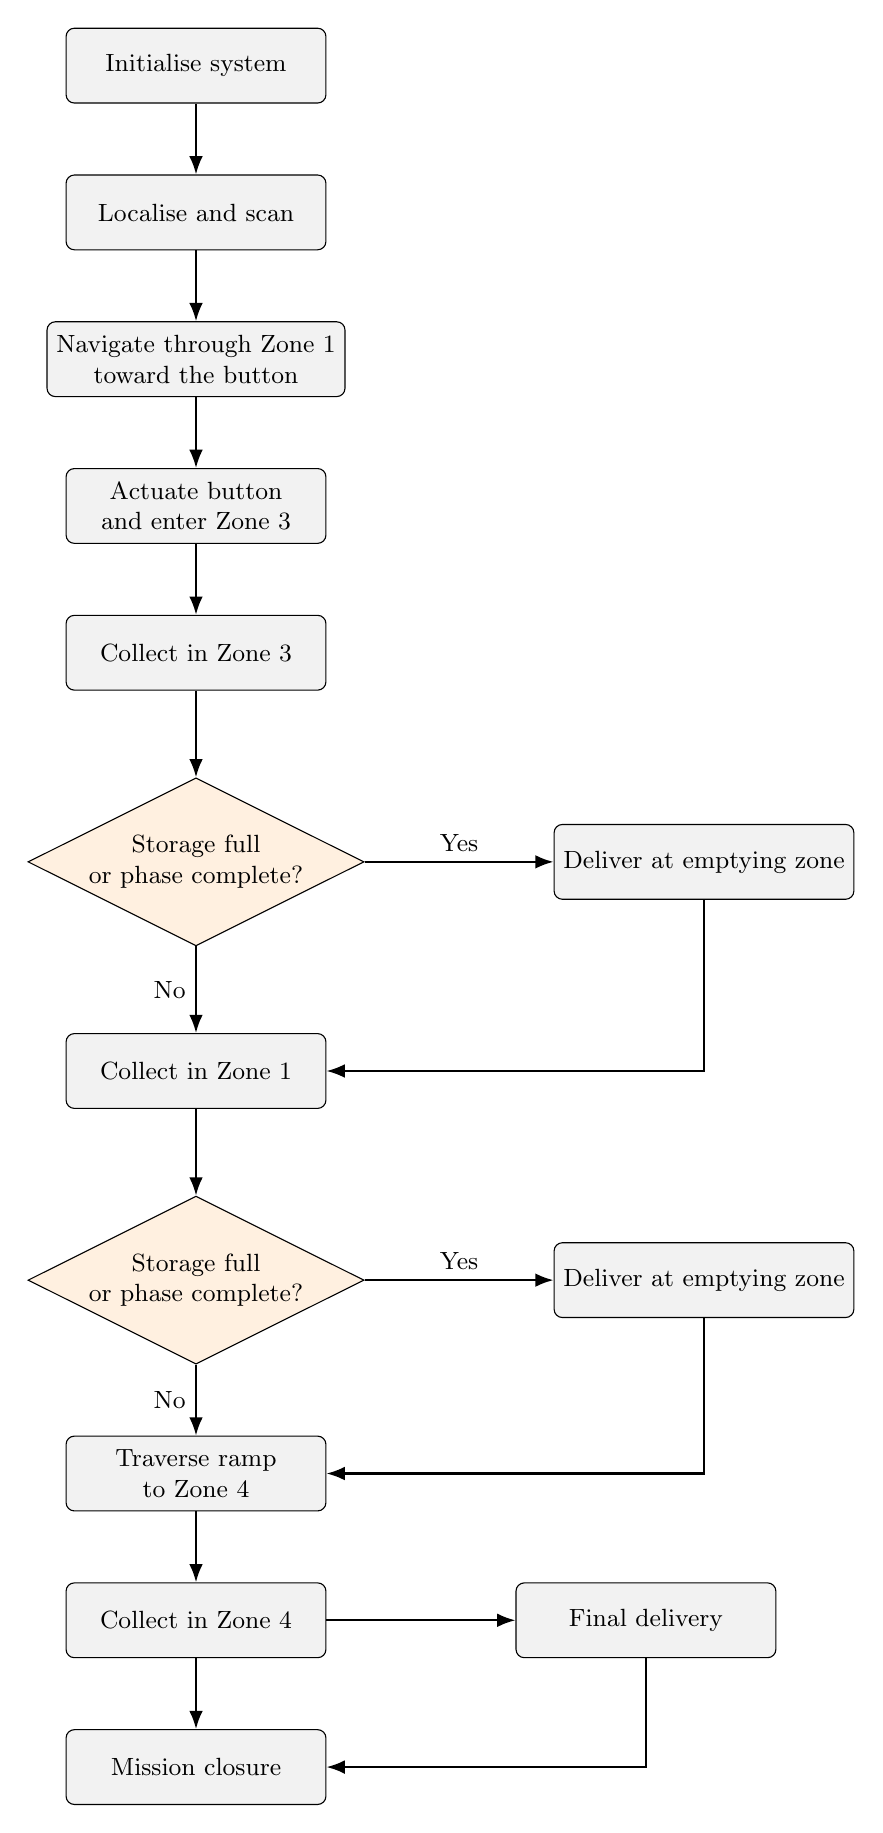
\begin{tikzpicture}[
  node distance=0.9cm and 1.2cm,
  every node/.style={font=\small},
  flowbox/.style={draw, rounded corners=3pt, align=center, fill=gray!10, minimum width=3.3cm, minimum height=0.95cm},
  decision/.style={draw, diamond, aspect=2, align=center, fill=orange!12, inner sep=1pt, minimum width=2.6cm},
  line/.style={-Latex, thick}
]
\node[flowbox] (init) {Initialise system};
\node[flowbox, below=of init] (loc) {Localise and scan};
\node[flowbox, below=of loc] (zone1) {Navigate through Zone 1\\toward the button};
\node[flowbox, below=of zone1] (button) {Actuate button\\and enter Zone 3};
\node[flowbox, below=of button] (zone3) {Collect in Zone 3};
\node[decision, below=1.1cm of zone3] (deliver1) {Storage full\\or phase complete?};
\node[flowbox, right=2.4cm of deliver1] (empty1) {Deliver at emptying zone};
\node[flowbox, below=1.1cm of deliver1] (zone12) {Collect in Zone 1};
\node[decision, below=1.1cm of zone12] (deliver2) {Storage full\\or phase complete?};
\node[flowbox, below=of deliver2] (ramp) {Traverse ramp\\to Zone 4};
\node[flowbox, right=2.4cm of deliver2] (empty2) {Deliver at emptying zone};
\node[flowbox, below=of ramp] (zone4) {Collect in Zone 4};
\node[flowbox, right=2.4cm of zone4] (final) {Final delivery};
\node[flowbox, below=of zone4] (stop) {Mission closure};

\draw[line] (init) -- (loc);
\draw[line] (loc) -- (zone1);
\draw[line] (zone1) -- (button);
\draw[line] (button) -- (zone3);
\draw[line] (zone3) -- (deliver1);
\draw[line] (deliver1) -- node[above]{Yes} (empty1);
\draw[line] (deliver1) -- node[left]{No} (zone12);
\draw[line] (empty1) |- (zone12);
\draw[line] (zone12) -- (deliver2);
\draw[line] (deliver2) -- node[above]{Yes} (empty2);
\draw[line] (deliver2) -- node[left]{No} (ramp);
\draw[line] (empty2) |- (ramp);
\draw[line] (ramp) -- (zone4);
\draw[line] (zone4) -- (stop);
\draw[line] (zone4) -- (final);
\draw[line] (final) |- (stop);
\end{tikzpicture}}
\caption{Operational functional flow of the robot during the competition: the planned mission sequence from localisation through the Zone~3, Zone~1, and Zone~4 legs to final delivery.}
\label{fig:functional_flow}
\end{figure}

\subsection{Functional Decomposition and motivated choices}
Each design space below includes several credible solutions with different trade offs. The comparison tables preserve the options considered and identify the selected solution. The realised implementations are described in Chapters~\ref{sec:mechanical}--\ref{sec:software}.

\subsubsection{Motion}
To move and turn in the arena, a planar drivetrain is required. Two main designs were studied, compared in Table~\ref{tab:movement_comparison}.

\begin{table}[H]
\centering
\small
\begin{tabularx}{\linewidth}{|P{0.16\linewidth}|P{0.16\linewidth}|Y|Y|Y|}
\hline
\textbf{Option} & \textbf{Principle} & \textbf{Advantages} & \textbf{Limitations} & \textbf{Relevance} \\
\hline
Differential drive (chosen) & Two actuated wheels and passive supports. & Low complexity and cost, simple integration, turns on the spot. & Non holonomic motion, more demanding motion modelling. & Best fit with the simplicity goal and the expected surfaces. \\
\hline
Omni wheel platform & Four omni wheels for holonomic motion. & Lateral manoeuvrability, easier target alignment. & Four actuators, higher mechanical complexity. & Attractive for precision but conflicts with the simplicity and power goals. \\
\hline
\end{tabularx}
\caption{Comparison of movement solutions.}\label{tab:movement_comparison}
\end{table}

After thorough comparison, a differential drive chariot with two high grip drive wheels and passive ball casters was selected, because it minimises the actuator count, allows turning on the spot for tight manoeuvres near bricks and walls, and integrates directly with the standard ROS~2 differential drive odometry and controller. Each drive wheel is closed loop speed controlled while the belt and fans run open loop; the realised control implementation (gains, feedforward, PWM frequency, and the encoder calibration) is described in the firmware section (Section~\ref{sec:firmware}).

\subsubsection{Collecting mechanism}
The collection function must capture bricks of variable size from the floor and feed them into storage. Three concepts were considered (Table~\ref{tab:grabbing_comparison}).

\begin{table}[H]
\centering
\small
\begin{tabularx}{\linewidth}{|P{0.13\linewidth}|P{0.18\linewidth}|Y|Y|Y|}
\hline
\textbf{Option} & \textbf{Principle} & \textbf{Advantages} & \textbf{Limitations} & \textbf{Relevance} \\
\hline
Compliant fans (chosen) & Two counter rotating fans with compliant blades pull bricks in. & High collection effectiveness, tolerant of brick shape, enables flow through collection. & Two actuators, careful intake dimensioning. & Highest ranked concept; matches the no stop strategy. \\
\hline
Passive ramp & Forward motion guides bricks up an inclined surface. & Very low complexity, no actuator. & Bricks may be pushed away instead of captured. & Low complexity but high performance risk. \\
\hline
Sweepers & Compliant rotating elements redirect bricks inward. & Mechanically compliant, impact tolerant. & Uncertain stiffness and efficiency. & Secondary concept if fans prove impractical. \\
\hline
\end{tabularx}
\caption{Comparison of block grabbing solutions.}\label{tab:grabbing_comparison}
\end{table}

The fan based intake was chosen because it enables a roomba style collection: rather than stopping at each brick, the robot drives through the brick positions and the front fans absorb them on the pass. This avoids precise stop and pick alignment, suits the differential drive, and keeps the ten minute budget productive. The selected design pairs the fans with an inclined ramp that redirects the captured bricks upward toward storage, so the ramp supports the fans rather than acting alone.

A risk analysis was conducted on the collection mechanism to assess potential failures and develop mitigation strategies, summarised in Table~\ref{tab:risk_collection}.

\begin{table}[H]
\centering
\small
\begin{tabularx}{\linewidth}{|Y|Y|c|c|Y|}
\hline
\textbf{Risk} & \textbf{Consequence} & \textbf{Likelihood} & \textbf{Level} & \textbf{Mitigation} \\
\hline
Brick bounces off the intake & Brick not collected & Med & Med & Compliant blades, drive through pass \\
\hline
Brick stuck at the entrance & Intake blocked & Med & Med & Wide intake, reverse fans to clear \\
\hline
Multiple bricks at once & Storage jam & Med & Low & Inclined ramp meters the flow \\
\hline
Fan reaction torque veers the robot & Heading drift while collecting & Med & Low & Counter rotating pair, heading hold control \\
\hline
\end{tabularx}
\caption{Risk analysis for the collection mechanism.}\label{tab:risk_collection}
\end{table}

\subsubsection{Storage and delivery}
Collected bricks must be stored during transport and released on command at the collection corner. The options are compared in Table~\ref{tab:delivery_comparison}.

\begin{table}[H]
\centering
\small
\begin{tabularx}{\linewidth}{|P{0.13\linewidth}|P{0.18\linewidth}|Y|Y|Y|}
\hline
\textbf{Option} & \textbf{Principle} & \textbf{Advantages} & \textbf{Limitations} & \textbf{Relevance} \\
\hline
Conveyor belt (chosen) & A motorised belt stores bricks and discharges them out the front on demand. & Fast, no reset motion, combines storage and release. & Needs ground clearance, one actuator, bearings. & Preferred: storage and delivery in one mechanism. \\
\hline
Motorised back door & An actuated hatch opens to release the payload. & Contains bricks, releases on command. & Extra actuator and hinge. & Viable but less favourable for repeated cycles. \\
\hline
PVC strip curtains & Passive flexible strips retain bricks until pushed out. & Simple, passive. & Light bricks may not generate enough force to exit. & Release reliability appears insufficient. \\
\hline
\end{tabularx}
\caption{Comparison of storage and delivery solutions.}\label{tab:delivery_comparison}
\end{table}

A conveyor belt was selected because it merges storage and delivery into a single actuator. Crucially, no separate back door or stepper actuation is required: to deliver, the belt direction and the fans are simply reversed, pushing the stored bricks back out the front. This reuses existing actuators and removes a failure prone hinge mechanism.

\subsubsection{Localisation and navigation}
Localisation must estimate the robot pose in the arena well enough to navigate to bricks, the button, and the collection corner. The candidate sensing and estimation concepts are compared in Table~\ref{tab:localization_comparison}.

\begin{table}[H]
\centering
\small
\begin{tabularx}{\linewidth}{|P{0.15\linewidth}|P{0.17\linewidth}|Y|Y|Y|}
\hline
\textbf{Option} & \textbf{Principle} & \textbf{Advantages} & \textbf{Limitations} & \textbf{Relevance} \\
\hline
LIDAR + SLAM (chosen) & Range sensing with simultaneous localisation and mapping. & High accuracy, direct wall based map. & Higher integration complexity. & Highest ranked localisation concept. \\
\hline
Sensor fusion (odom + IMU + LIDAR) (chosen) & Fuse proprioceptive and exteroceptive measurements. & Redundant, robust to single sensor weaknesses. & More implementation effort. & Adopted on top of SLAM for robust short term odometry. \\
\hline
Wheel odometry & Integrate wheel encoder motion. & Simple, self contained. & Drifts, sensitive to slip. & Baseline input to the fusion. \\
\hline
IMU & Inertial heading and motion cues. & Heading without wheel ground assumptions. & Position drifts over time. & Complementary, not standalone. \\
\hline
Visual markers & Known markers as absolute references. & Absolute corrections when visible. & Limited range, light sensitive. & Not robust enough as primary. \\
\hline
\end{tabularx}
\caption{Comparison of localisation solutions.}\label{tab:localization_comparison}
\end{table}

Taking into account the requirement to navigate an $8 \times 8$~m arena with walls, it was concluded that a 2D LIDAR feeding a SLAM map, combined with an Extended Kalman Filter fusing wheel odometry and the IMU for the short term \texttt{odom} frame, was the most effective solution: the LIDAR gives accurate wall based mapping and the fusion gives smooth, drift bounded odometry between LIDAR corrections. The realised stack, including the EKF fusion design, the choice of SLAM package, AMCL localisation, and the IMU calibration, is detailed in Section~\ref{sec:highlevel}.

A risk analysis for localisation and navigation is given in Table~\ref{tab:risk_nav}.

\begin{table}[H]
\centering
\small
\begin{tabularx}{\linewidth}{|Y|Y|c|c|Y|}
\hline
\textbf{Risk} & \textbf{Consequence} & \textbf{Likelihood} & \textbf{Level} & \textbf{Mitigation} \\
\hline
SLAM divergence & Loss of global reference & Low & High & AMCL re-initialised at the known base pose \\
\hline
TF frame mismatch & Robot moves to wrong coordinates & Low & High & Validated transform tree, single TF owner per edge \\
\hline
Wheel slip on fast pivots & Yaw over read by odometry & Med & Med & Gyro is the sole yaw source in the EKF \\
\hline
Path planner oscillation & Time wasted re-planning & Med & Low & Velocity floors and tuned costmap inflation \\
\hline
\end{tabularx}
\caption{Risk analysis for localisation and navigation.}\label{tab:risk_nav}
\end{table}

\subsubsection{Brick and obstacle detection}
The perception sensor must support both brick detection and obstacle ranging. The options are compared in Table~\ref{tab:perception_sensing_comparison}.

\begin{table}[H]
\centering
\small
\begin{tabularx}{\linewidth}{|P{0.13\linewidth}|P{0.17\linewidth}|Y|Y|Y|}
\hline
\textbf{Option} & \textbf{Principle} & \textbf{Advantages} & \textbf{Limitations} & \textbf{Relevance} \\
\hline
Depth camera (chosen) & One sensor gives colour and range. & Brick detection and distance from one stream. & Higher cost, moderate processing load. & Preferred for combined detection and ranging. \\
\hline
LIDAR (chosen for obstacles) & Laser ranging of obstacle geometry. & Accurate, wide field of view, long range. & Brick discrimination is indirect. & Adopted specifically for obstacle avoidance. \\
\hline
Camera + processing & Monocular imaging with vision algorithms. & Flexible, low sensor cost. & Light sensitive, no direct depth. & Less robust than depth sensing. \\
\hline
Infrared / ultrasonic & Short range proximity sensing. & Inexpensive, simple. & Narrow field, very short range. & Only supplemental. \\
\hline
\end{tabularx}
\caption{Comparison of detection sensing solutions.}\label{tab:perception_sensing_comparison}
\end{table}

A depth camera (OAK-D Lite) was chosen for brick detection because it provides colour and aligned depth from a single device, allowing a detected brick centroid to be projected directly to a 3D position, and because its Myriad X VPU offloads the stereo depth computation from the host CPU. A 2D LIDAR was retained in parallel for obstacle detection and the SLAM map, since implementing it with the ROS~2 navigation stack requires minimal effort and it provides an accurate, wide field of view range measurement that the camera cannot. The driver level constraints this sensor imposed (RGB aligned depth, the mandatory pipeline and IMU synchronisation settings) are covered in the software section.

For the detection algorithm itself, two software approaches were compared (Table~\ref{tab:block_detection_comparison}).

\begin{table}[H]
\centering
\small
\begin{tabularx}{\linewidth}{|P{0.16\linewidth}|P{0.18\linewidth}|Y|Y|Y|}
\hline
\textbf{Option} & \textbf{Principle} & \textbf{Advantages} & \textbf{Limitations} & \textbf{Relevance} \\
\hline
OpenCV HSV detection & Classical colour segmentation plus contour and centroid tracking. & Low overhead, near zero latency, deterministic. & Sensitive to lighting; fails when ambient light changes. & Used as an intermediate solution; later dropped for poor lighting robustness. \\
\hline
Deep learning (YOLO, on VPU) (chosen) & Trained neural network detector running on the OAK VPU. & Robust to lighting once trained; runs on device. & Needs a correct training and deployment pipeline. & Final detector after retraining; runs on the VPU without host CPU cost. \\
\hline
\end{tabularx}
\caption{Comparison of brick detection software approaches.}\label{tab:block_detection_comparison}
\end{table}

The detector went through several iterations during the project (YOLO, then HSV, then a retrained YOLO on the camera VPU), which is one of the more instructive software stories and is discussed in Section~\ref{sec:vision}.

\subsubsection{Compute platform, power, and middleware}
The computing platform, the power architecture, and the software middleware were each selected from the options in Tables~\ref{tab:hardware_comparison}--\ref{tab:middleware_comparison}. ROS~2 Humble with Nav2 was adopted as the middleware for its long term support, its reusable navigation and SLAM packages, and its DDS transport; the power architecture supplies the motors directly from the battery with a regulated 5~V rail for the electronics; and an NVIDIA Jetson Nano was chosen as the on board computer for its nominal GPU acceleration. How these choices were realised, the problems encountered, and how the outcome differed from this plan, in particular why the Jetson choice proved to be a mistake, are detailed in Chapters~\ref{sec:electrical} and \ref{sec:software}.

\begin{table}[H]
\centering
\small
\begin{tabularx}{\linewidth}{|P{0.16\linewidth}|Y|Y|Y|}
\hline
\textbf{Option} & \textbf{Advantages} & \textbf{Limitations} & \textbf{Relevance} \\
\hline
Raspberry Pi & Simple ROS integration, compact. & Limited compute for heavy perception. & Initial baseline. \\
\hline
NVIDIA Jetson Nano (chosen) & GPU/VPU capacity for perception. & Higher cost and power. & Adopted once the stack exceeded the Pi. \\
\hline
\end{tabularx}
\caption{Comparison of on board computing platforms.}\label{tab:hardware_comparison}
\end{table}

\begin{table}[H]
\centering
\small
\begin{tabularx}{\linewidth}{|P{0.18\linewidth}|Y|Y|Y|}
\hline
\textbf{Option} & \textbf{Advantages} & \textbf{Limitations} & \textbf{Relevance} \\
\hline
Battery for motors + one 5~V rail (chosen) & Simple, satisfies the 5~V digital requirement. & Restricts electronics to 5~V regulation. & Preferred: minimal power system complexity. \\
\hline
Battery + multiple regulated rails & Supports more component voltages. & More complex. & Only if sensors need other rails. \\
\hline
Single regulated 5~V for everything & Uniform architecture, stable motor speed. & Limits motors, high regulator current. & Only for a very small platform. \\
\hline
\end{tabularx}
\caption{Comparison of power architecture options.}\label{tab:power_comparison}
\end{table}

\begin{table}[H]
\centering
\small
\begin{tabularx}{\linewidth}{|P{0.16\linewidth}|Y|Y|Y|}
\hline
\textbf{Option} & \textbf{Advantages} & \textbf{Limitations} & \textbf{Relevance} \\
\hline
ROS~2 with Nav2 (chosen) & Robust, modular, industry aligned. & Steeper learning curve. & Best match for integrating the full stack. \\
\hline
ROS~1 & Large community. & Obsolete relative to ROS~2. & Fallback only. \\
\hline
Custom DDS layer & Full control. & Not realistic in the schedule. & Incompatible with the timeline. \\
\hline
\end{tabularx}
\caption{Comparison of middleware and software architecture options.}\label{tab:middleware_comparison}
\end{table}

% =====================================================================
\section{Mechanical design}\label{sec:mechanical}
% =====================================================================

The mechanics must enable the functions established above: stable differential drive motion, ground clearance and traction for the ramp, a low intake for collection across brick sizes, internal storage, controlled delivery, and a rigid contact element for the button. The realised structure is shown in CAD and as the assembled robot in Figure~\ref{fig:chassis_rear_iso}.

\reportfig{back_assembly.png}{0.8}{Isometric rear view of the assembled chassis, showing the drive wheel integration, upper electronics housing, and sensor mounting points.}{fig:chassis_rear_iso}

\subsection{Structure design}

\subsubsection{Chassis specifications}
The robot's chassis is a multi-tier frame constructed from laser-cut medium-density fibreboard (MDF), selected for its cost-efficiency, rapid manufacturability, and adequate structural rigidity under expected dynamic loads. To achieve the necessary strength to withstand operational stresses, the MDF panels were permanently assembled using adhesive bonding on interlocking laser-cut box joints, as shown on \ref{fig:chassis_frame}. The architecture is divided into two primary functional levels. The lower tier integrates the mobility and collection systems, housing the drive motors alongside a ground-level intake mechanism that features a propeller-assisted ramp and a conveyor belt.

The upper tier accommodates the electronics payload—including the on-board computer, motor controllers, and power distribution—while serving as the mounting platform for the sensor suite. Sensor placement is optimized for maximum spatial awareness: the LIDAR is elevated to ensure an unobstructed 360° scanning plane, and the camera is mounted on a forward mast angled downward. This camera positioning ensures that target bricks enter the field of view immediately preceding the intake trajectory.

\reportfig{frame.png}{0.7}{Bare MDF chassis frame with interlocking laser-cut box joints}{fig:chassis_frame}



\subsubsection{Ramp ground clearance}
The geometric design of the chassis was driven by two competing constraints: maximizing the underbody clearance to navigate the arena's ramp without interference, while minimizing the intake height to successfully capture flat-lying bricks. Specifically, the lower chassis profile had to maintain a strict clearance envelope, defined by 30° approach and departure angles extending from the wheel contact points and connected by a central clearance arc. To satisfy these requirements, the lowest edge of the collection ramp was precisely aligned with the contact plane of the passive wheels. Furthermore, to accommodate real-world manufacturing tolerances, the passive wheels were mounted within vertically slotted grooves, allowing their elevation to be fine-tuned via screw fasteners after assembly.

This complex spatial relationship was validated using a detailed 2D side-profile schematic, shown in Figure~\ref{fig:ramp_clear}. The geometric constraints of the chassis are defined by the wheelbase ($L$) and the ground clearance ($c$). To ensure the robot can navigate the crest of the ramp without high-centering, the breakover angle ($\beta$) and the clearance arc radius ($R$) were calculated. 

Given the initial design parameters of $L = 30\text{ cm}$ and $c = 2.5\text{ cm}$, the breakover angle is determined by:

\begin{align}
    \beta &= 2 \arctan\left(\frac{2c}{L}\right) \nonumber \\
    \beta &= 2 \arctan\left(\frac{2 \times 2.5}{30}\right) \approx 18.9^\circ
\end{align}

Similarly, the radius of the clearance arc bounding the undercarriage is calculated as:

\begin{align}
    R &= \frac{c}{2} + \frac{L^2}{8c} \nonumber \\
    R &= \frac{2.5}{2} + \frac{30^2}{8 \times 2.5} = 46.25 \text{ cm}
\end{align}

Because the required breakover capacity ($\beta \approx 18.9^\circ$) safely exceeded the competition ramp's actual crest angle of $17.5^\circ$, the geometric layout was deemed viable for fabrication.

\reportfig{Ramp clearance.png}{0.7}{2D side-profile schematic, showing the required ground clearance to pass the ramp}{fig:ramp_clear}


\subsection{Drivetrain and navigation}

\subsubsection{Actuator choice}
To reduce the electronics architecture complexity, a unified actuator strategy was adopted. The identical geared DC motors (DFRobot FIT0403, $90{:}1$ nominal reduction) used for the main drivetrain were also selected for the internal mechanisms. 

Mobility is provided by a differential drive system utilizing wide, high-grip $120\times60\text{ mm}$ wheels (Wild Thumper) spaced at a track width of $28\text{ cm}$. This track width dictates the in-place rotation radius and provides the baseline for the odometry kinematics. To enable smooth, omnidirectional pivoting during differential steering without introducing lateral drag, the front passive supports utilize industry-grade ball casters. 

\subsubsection{Kinematics and torque validation}
Based on the manufacturer specifications of $122\text{ rpm}$ under no-load conditions and the wheel radius of $r = 0.06\text{ m}$, the theoretical maximum angular velocity ($\omega_{\text{max}}$) and linear chassis speed ($v_{\text{max}}$) were calculated. Under physical load, the nominal running speed drops to approximately $11\text{ rad/s}$, providing a highly controllable effective top speed of $0.66\text{ m/s}$.

\begin{align}
    \omega_{\text{max}} &= 122 \text{ rpm} \times \frac{2\pi}{60} \approx 12.78 \text{ rad/s} \\
    v_{\text{max}} &= \omega_{\text{max}} \times r = 12.78 \text{ rad/s} \times 0.06 \text{ m} \approx 0.77 \text{ m/s}
\end{align}

To verify the drivetrain's capacity to ascend the 30° arena ramp, the required climbing torque was calculated and compared against the manufacturer's rated stall torque for the actuators. According to the technical specifications, each motor provides a maximum stall torque of $38\text{ kg}\cdot\text{cm}$. Converting this to standard SI units yields an available torque ($\tau_{\text{avail}}$) of approximately $3.73\text{ N}\cdot\text{m}$:

\begin{align}
    \tau_{\text{avail}} &= 38\text{ kg}\cdot\text{cm} \times \left(0.01\text{ m/cm}\right) \times 9.81\text{ m/s}^2 \nonumber \\
    \tau_{\text{avail}} &\approx 3.73\text{ N}\cdot\text{m}
\end{align}

The required climbing torque must overcome the gravitational force ($F_{\text{climb}}$) acting parallel to the incline. With a total robot mass of $m = 10\text{ kg}$, this force is:

\begin{align}
    F_{\text{climb}} &= m \cdot g \cdot \sin(30^\circ) \nonumber \\
    F_{\text{climb}} &= 10 \cdot 9.81 \cdot 0.5 = 49.05\text{ N}
\end{align}

With dual drive motors, the required driving torque per motor ($\tau_{\text{req}}$) to maintain forward equilibrium is calculated as:

\begin{align}
    \tau_{\text{req}} &= \frac{F_{\text{climb}} \cdot r}{2} \nonumber \\
    \tau_{\text{req}} &= \frac{49.05 \cdot 0.06}{2} \approx 1.47\text{ N}\cdot\text{m}
\end{align}

Because the available stall torque per motor ($3.73\text{ N}\cdot\text{m}$) is significantly greater than the required climbing torque ($1.47\text{ N}\cdot\text{m}$), the actuators possess sufficient mechanical capacity to overcome the incline.

\reportfig{bottom_assembly.png}{0.9}{Bottom view of the assembly illustrating the front ball casters and the rear-mounted wheel actuators.}{fig:chassis_bottom}

\subsection{Collecting mechanism}


The intake mechanism consists of two counter-rotating fans with compliant blades positioned at the front of the robot, flanking a 30° inclined ramp. Inspired by the functional architecture of the BlockBuster robot (Team 5, 2024), the system operates by pulling bricks inward while the ramp guides them upward onto the conveyor belt. The compliant nature of the blades allows the mechanism to conform to various brick shapes and sizes without inflicting damage, satisfying the strict brick integrity requirements. The propellers are mounted in a mirrored configuration; a positive command drives them inward for collection, while reversing the rotation expels the bricks during the delivery phase. The final system includes inclined flanges to constrain blocks on the top of the conveyor belt, as shown on \ref{fig:chassis_cross_section}.


\reportfig{half_assembly.png}{0.9}{Cross-sectional view detailing the internal architecture, including the 5-blade intake propeller, collection ramp, and Dycem conveyor belt mechanism.}{fig:chassis_cross_section}

Initial testing revealed critical reliability issues. The primary failure mode occurred when bricks became tightly wedged between the propellers. Once a block jammed and forced the system to stall, the motors lacked the necessary starting torque to overcome static friction and push the stationary block up the incline. While early hypotheses attributed this to the blade count or curvature, observations of varying blade setups showed no measurable improvement. 

Instead, empirical testing demonstrated that capture efficiency was fundamentally constrained by the intake's spatial geometry and material properties. To resolve the jamming, the robot chassis was redesigned to significantly increase the internal width and the distance between the two propellers, allowing bricks to pass through more freely. Furthermore, the propeller assemblies were structurally optimized: the central axles were manufactured from rigid PETG to maximize torque transmission from the motors, while the blades themselves were printed in flexible TPU to retain the necessary compliance. Additionally, the collection ramp was redesigned as a 3D-printed component to achieve a significantly sharper leading edge, reducing the initial kinetic barrier encountered by flat-lying bricks. A summary of these geometric optimizations is detailed in Table~\ref{tab:intake_specs}.

Due to time constraints preventing further isolated optimization on blade counts, a five-blade configuration was adopted for the final iteration. These final blades were designed with a straight, non-curved profile. Because the propellers must rotate in both directions (inward for intake, outward for delivery), curved aerodynamic profiles offer no proven benefit and would behave asymmetrically.

\begin{figure}[htbp]
    \centering
    \begin{minipage}{0.48\textwidth}
        \centering
        \includegraphics[width=\linewidth]{images/intakeV1.png}
        \caption{Original intake design, which suffered from narrow spacing and a higher ramp.}
        \label{fig:intake_v1}
    \end{minipage}\hfill
    \begin{minipage}{0.48\textwidth}
        \centering
        \includegraphics[width=\linewidth]{images/intakeV2.png} 
        \caption{Latest intake design, featuring a widened chassis, extended blades, and a lowered ramp.}
        \label{fig:intake_v2}
    \end{minipage}
\end{figure}


\begin{table}[htbp]
    \centering
    \caption{Comparison of original (v1) and optimized (v2) intake specifications.}
    \label{tab:intake_specs}
    \renewcommand{\arraystretch}{1.2}
    \begin{tabular}{lcc}
        \hline
        \textbf{Parameter} & \textbf{Version 1} & \textbf{Version 2} \\
        \hline
        Propeller axle distance & 13.0 cm & 17.0 cm \\
        Effective clearance (minus propeller width) & 11.5 cm & 14.0 cm \\
        Blade length (from center of rotation) & 5.0 cm & 7.0 cm \\
        Blade width & 3.0 mm & 6.0 mm \\
        Internal chassis width & 25.0 cm & 33.0 cm \\
        Ramp thickness & 8.5 mm & 5.0 mm \\
        \hline
    \end{tabular}
\end{table}

\subsection{Storage and delivery mechanism}
\subsubsection{Conveyor Belt}
To transition from the intake mechanism to the storage bay, a motorised floor conveyor belt was developed. Unlike the reference BlockBuster design, which relied solely on fan-based intake and a separate mechanism for output, this conveyor serves a dual purpose: accumulating bricks during collection and actively discharging them during delivery. During the collection phase, the fans pull the bricks upward where they naturally accumulate on the static belt inside the storage volume. While early designs anticipated needing intermittent belt actuation to clear space at the front of the intake, testing revealed this was unnecessary, allowing for a simplified, unactuated collection state. During the delivery phase, the system reverses: the conveyor belt is actuated forward, carrying the stored bricks into the fans, which are simultaneously reversed to expel the payload out the front of the chassis. This shared intake/output architecture eliminates the need for complex secondary actuators or hinged trapdoors.

\subsubsection{Belt material and joining}
The conveyor surface requires a high coefficient of friction to reliably transport the smooth plastic bricks. Taking inspiration from the Robocop robot (Team 3, 2025), a medical-grade anti-slip polymer known as Dycem was selected. While their team utilized Dycem on a steep incline before pivoting to a vertical lift, our horizontal floor configuration proved ideal for the material's high-grip properties. 

Constructing a continuous loop from the Dycem sheet presented manufacturing challenges. Initial attempts using double-sided adhesive tape failed under dynamic tension after only a few test runs. To achieve a durable, tension-resistant loop, the ends of the material were permanently joined using structural sewing. 

\subsubsection{Rollers and power transmission}
The conveyor belt is tensioned across two custom 22\,mm diameter 3D-printed rollers. The original design called for a multi-material roller consisting of a structural steel core, a standard PVC pipe outer shell, and 3D-printed interface hubs. However, due to regional supply chain limitations regarding PVC pipe dimensions, the outer shell was fully transitioned to a 3D-printed component. 

Power is transmitted to the driving roller via a secondary transmission belt sourced from MISUMI. Custom 3D-printed pulleys were designed to interface with this belt, which were subsequently updated to include high-walled side grooves (flanges) to prevent the belt from derailing under load. A ball-bearing tensioner is utilized to maintain optimal belt engagement. 

The rollers rotate on 8\,mm diameter steel axles supported by 8\,mm inner-diameter ball bearings, which are mounted to the chassis via custom 3D-printed brackets. Due to unoptimized tolerance matching between the axle and bearing bore, an interference fit was achieved using hammering. While this severely limited the ease of disassembly, it provided the benefit of locking the components axially, eliminating the need for retaining rings to prevent lateral drift during operation.

\reportfig{conveyor.png}{0.85}{Conveyor belt mechanism showing the 3D-printed rollers, Dycem belt, and transmission system.}{fig:conveyor}

\paragraph{Recommendation for future teams.}
\begin{itemize}[noitemsep]
    \item Test the mechanical functions early and independently, before the full chassis exists. A very simple bench rig (a battery and two cables driving a motor directly) is enough to validate the intake, the conveyor, or a wheel against real bricks and to catch problems while they are still cheap to fix.
    \item Adapt the structure to the functional parts, not the reverse; this follows naturally from testing the functional parts first.
    \item If a validated prior design is taken as the starting point, reproduce it faithfully before attempting variations. Concretely, the reference collector used two large five blade fans; three blade and then two blade variants were tried first, failed to capture bricks reliably, and the original five blade configuration was finally adopted, at which point the intake worked. The reduced blade counts brought no measurable benefit.
    \item Either reuse a tested design as is, or commit to a genuinely original route, but do not copy an architecture while discarding the implementation details that made it work.
\end{itemize}


% =====================================================================
\section{Electrical design}\label{sec:electrical}
% =====================================================================

\subsection{Components overview and motivations}
The electronics were selected to satisfy the autonomy, on board computation, and on board power requirements, and to drive the five motors of the platform. The major components and their motivations are:
\begin{itemize}[noitemsep]
    \item \textbf{On board computer: NVIDIA Jetson Nano.} A first generation Jetson Nano was selected for its industry oriented platform and its nominal GPU acceleration, with the intention of offloading the heavy perception computation onto the GPU. It runs ROS~2 Humble inside a Docker container. As discussed below and in Section~\ref{sec:swlessons}, this choice turned out to be a mistake for this workload.
    \item \textbf{Camera: Luxonis OAK-D Lite.} Chosen for brick detection because it provides RGB plus aligned stereo depth, with an on device Myriad X VPU that offloads stereo depth generation from the host. An external IMU had originally been budgeted, but it was dropped once it was discovered that this OAK-D unit already integrated a BMI270 IMU (not all OAK-D units in the cohort did). Because that BMI270 is only a 6 axis sensor with no magnetometer, yaw is not directly observable; acceptable accuracy was nonetheless recovered in software through a per run calibration (Section~\ref{sec:loc}), although a dedicated 9 axis IMU would have been the better choice when yaw accuracy matters.
    \item \textbf{LIDAR: RPLidar A1M8.} A low cost $360^\circ$ 2D LIDAR used for SLAM and obstacle avoidance, with a reliable indoor range of about $6$--$10$~m and a scan rate near $7.5$~Hz, which is well matched to an $8 \times 8$~m arena.
    \item \textbf{Microcontroller: ESP32.} A dedicated real time microcontroller runs the motor control firmware and communicates with the Jetson over micro-ROS on a serial link. Offloading the time critical PWM and encoder handling to the ESP32 keeps motor control deterministic regardless of the Linux scheduler. Two boards were obtained so that a spare was always available, since a reflash failure or a damaged board would otherwise halt all motor control. The ESP32 pinout used is shown in Figure~\ref{fig:esp32}.
    \item \textbf{Motor driver: DC Motor Driver 2x15A Lite.} A PWM plus direction H bridge rated $15$~A per channel, far above the few amperes the motors draw, providing margin against stall currents. The PWM frequency was set to $21$~kHz: above the audible range and below the driver's $25$~kHz switching cap.
    \item \textbf{Actuators: five motors.} Two geared DC drive motors with quadrature encoders (closed loop speed control), one belt motor, and two fan motors (open loop). The encoders provide $5756$ counts per output revolution after calibration, used for wheel odometry.
\end{itemize}

\reportfig{esp32pinout.png}{0.7}{ESP32 development board pinout used for the motor control firmware (PWM and direction lines, encoder inputs).}{fig:esp32}

\subsection{Computing platform}
The computation is split across three elements. The Jetson Nano runs the full ROS~2 Humble autonomy stack (perception, localisation, navigation, and mission logic) inside a Docker container. The ESP32 runs the low level motor firmware (Section~\ref{sec:firmware}) and exposes it to ROS~2 through a micro-ROS agent over a serial link. Finally, the OAK-D camera's Myriad~X VPU runs the stereo depth generation, and optionally the on device brick detector, so the host CPU is not burdened with that computation. In hindsight the Jetson Nano was the wrong choice for this workload: the ROS~2 navigation stack is CPU bound rather than GPU bound, so its nominal GPU went unused while its $4$~GB of RAM and thermal limits throttled the full stack and made it the pipeline bottleneck, where a Raspberry Pi~5 would have served better (revisited in Section~\ref{sec:swlessons}).

\subsection{Motor and driver selection}
The motors were sized against the load on each wheel and the wheel radius. With a total robot mass near $5$~kg shared over the two driving wheels, roughly $2.5$~kg bears on each, and the tractive force needed to drive a wheel on the flat is of the order $F \approx 2.5$~N. For a wheel radius $r \approx 0.06$~m this gives a per motor operating torque
\begin{equation*}
M = F\,r \approx 2.5 \times 0.06 \approx 0.18~\text{N\,m}.
\end{equation*}
The selected gearing turns the output near $114$~rpm, that is $\omega = 114 \cdot 2\pi/60 \approx 11.9$~rad/s, for a ground speed $v = \omega\,r \approx 0.6$~m/s. The bare motor is rated near $24.5$~mN\,m at its $9$~V, $2060$~rpm point drawing about $1$~A, which the gearbox multiplies comfortably past the flat ground operating torque. The ramp is the worst case: a contact analysis at the ramp angle pushed the demanded torque up to the order of a few N\,m, so the ramp, not flat driving, was identified early as the torque limited manoeuvre, with traction and ground clearance the binding constraints. Rather than the Maxon motors common in the cohort, a cheaper geared DC motor with an integrated quadrature encoder was chosen~\cite{dfrobotmotor}: it met the computed torque and speed requirements at a fraction of the cost while still providing the encoder feedback the closed loop wheel control needs. The same motor model was used for all five actuators, including the belt and the two fans, even though those run open loop. This was deliberate: the belt and fans only need to be switched on and off at full speed and reversed in direction, to take blocks in during collection and push them out during delivery, so tuning a controller for them would have wasted time for no benefit, while a single motor model simplified spares and wiring.

The cost saving shifted effort onto the driver and the firmware. The chosen DC Motor Driver 2x15A Lite~\cite{dfrobotdriver} exposes only a simple PWM plus direction interface and, unlike a Maxon controller, has no built in control loop at the driver level. Much of the firmware effort therefore went into implementing precise speed control on the ESP32 itself, the PI loop, the model based feedforward, and the active braking described in Section~\ref{sec:firmware}, to recover the closed loop behaviour an integrated motor controller would have provided out of the box.

The drivetrain feedback comes from the motor's integrated quadrature encoder, decoded in hardware on the ESP32. The motor has a nominal $16$ counts per revolution at the shaft behind a $90{:}1$ gearbox, which gives $1440$ counts per output revolution, or $5760$ in full ($4\times$) quadrature. The figure actually used in both the firmware and the host odometry was the measured one, $5756$ ticks per wheel revolution (about $916.1$ ticks per radian), because the nominal value drifts the integrated distance over a long run. The two wheel encoders are read through the ESP32 PCNT peripheral with a $1~\mu\text{s}$ glitch filter, which rejects the PWM switching noise that would otherwise add false counts while the wheel is stationary, and a hardware accumulator extends the $16$ bit counter so revolutions are never lost. One interfacing detail had to be resolved at assembly: the encoders output their quadrature signals at $5$~V logic, whereas the ESP32 GPIOs are $3.3$~V, so bidirectional logic level shifters were added on the soldered breadboard to bring the encoder lines down to the microcontroller's level. Powering the encoders from $3.3$~V instead would have avoided the shifters, but the ESP32 board's onboard LDO only supplies the microcontroller itself and no separate $5$~V to $3.3$~V converter was on hand for the encoders, so level shifting was the simpler route given the available parts.

\subsection{Power system and current budget}
The power architecture supplies the motors directly from the battery (VBAT) and provides regulated $5$~V rails for the digital electronics, which satisfies the mandatory $5$~V digital requirement. Supplying the motors at battery voltage keeps the current path short and avoids loading the regulators with the high transient motor currents, while the regulated rails power the Jetson, the ESP32, the LIDAR, and the camera. The H bridge channels are rated well above the motor running current so that ramp climbing stall transients do not exceed the driver limits. The complete electrical schematic, documenting all interconnections between the battery, the regulators, the driver, the ESP32, and the sensors, is given in Figure~\ref{fig:schematic}.

\vecfig{schematic}{0.95}{Complete electrical schematic: battery, 5~V regulation, motor driver, ESP32, and sensor interconnections.}{fig:schematic}

The consumption budget was used to size the regulation and the wiring. It has to be expressed in power rather than current, because the five motors are fed directly at the battery voltage (about $11.1$~V) while the computer and the digital electronics sit on the regulated $5$~V rail, so their currents are drawn at different voltages and cannot be compared directly. The budget at the nominal operating point is summarised in Table~\ref{tab:current}. The drive and intake motors dominate it and are by far the most variable: each draws only about $0.66$~A at the nominal operating torque but up to $7$~A at full stall, which is why the $15$~A per channel driver was retained.

\begin{table}[H]
\centering
\small
\begin{tabularx}{\linewidth}{|Y|c|c|c|}
\hline
\textbf{Load} & \textbf{Rail} & \textbf{Current} & \textbf{Power} \\
\hline
Motors (5, operating) & VBAT ($11.1$~V) & $3.3$~A ($0.66$~A each) & $36.7$~W \\
\hline
Jetson Nano & $5$~V & $4.0$~A & $20.0$~W \\
\hline
Sensor and logic board & VBAT ($11.1$~V) & $0.5$~A & $5.6$~W \\
\hline
\textbf{Total (nominal)} & --- & --- & \textbf{$62.3$~W} \\
\hline
\end{tabularx}
\caption{Power budget at the nominal operating point. The motors are measured at the battery rail and the Jetson at the $5$~V rail, so the loads are compared by power, not by current. The five motors together range from about $1.75$~A with no load ($19.5$~W) to $35$~A at full stall ($388.5$~W).}\label{tab:current}
\end{table}


At the time this budget was drawn up, the plan was a single regulated $5$~V rail feeding everything digital, with no separate converter for the computer. That design proved too naive precisely on this rail. During integration the Jetson began shutting off, seemingly at random but in practice correlated with the first runs in which the camera and the LIDAR streamed at the same time. The cause was a current shortfall: with the camera and the LIDAR both drawing over USB on top of the encoders, the motor drivers, and the ESP32, the shared rail could no longer supply the Jetson with the current it needed, and the computer browned out and reset. The fix was to put the Jetson on its own simple DC/DC converter, isolated from the rest of the digital load, which removed the shutdowns entirely.

\paragraph{Power budget and autonomy.} The drive motor current was modelled linearly between the measured no load and stall points, $I(\tau) = I_0 + (I_\text{stall} - I_0)\,\tau/\tau_\text{stall}$, with $I_0 \approx 0.35$~A and $I_\text{stall} \approx 7$~A per motor. At the $0.18$~N\,m operating torque this gives about $0.66$~A per motor, so the five motors together draw roughly $3.3$~A at the $11.1$~V pack, about $37$~W. Adding the Jetson (about $20$~W) and the sensor and logic board (about $5.6$~W, drawn at the battery rail) brings the total continuous draw to about $62$~W (Table~\ref{tab:current}). The battery is a $3$S LiPo ($12.6$~V full, $11.1$~V nominal, $9.9$~V cutoff) of $4$~Ah, that is $44.4$~Wh, of which about $85\%$ is usable down to the safe state of charge, leaving about $37.7$~Wh. The estimated autonomy is therefore
\begin{equation*}
t = \frac{37.7~\text{Wh}}{62~\text{W}} \approx 0.6~\text{h} \approx 36~\text{min},
\end{equation*}
comfortably above the ten minute competition run, with margin for the bursty stall transients that the linear average does not capture.

\subsection{Low level firmware}\label{sec:firmware}
The motor control is handled entirely by the ESP32 firmware, which runs five motor tasks under FreeRTOS and is exposed to the ROS~2 stack through a micro-ROS agent over a serial link~\cite{microros}. Placing this layer on a dedicated microcontroller, rather than on the Linux host, keeps the PWM generation and the encoder counting deterministic regardless of the Jetson's scheduler load, and it is the layer most directly responsible for the robustness of the platform. Its task structure is shown in Figure~\ref{fig:firmware}.

\vecfig{firmware}{0.95}{ESP32 firmware architecture: five FreeRTOS motor tasks communicate with the micro-ROS task only through the lock free \texttt{AppBus} channels; the wheels run closed loop PI on encoder feedback while the belt and fans run open loop, and the safety gates force every motor to zero under any fault.}{fig:firmware}

\paragraph{Thread-safe communication (AppBus).} The six FreeRTOS tasks (the micro-ROS task and the five motor tasks) never share mutable state directly; they exchange data only through the \texttt{AppBus}, a set of typed single-direction queues (\texttt{Channel<T>}, each backed by a FreeRTOS queue). For every motor there is one pair: \texttt{to\_motor[id]} carries a \texttt{MotorCmd} written only by the micro-ROS task and read only by that motor's task, while \texttt{from\_motor[id]} carries a \texttt{MotorFeedback} written only by the motor task and read only by the micro-ROS task. Because each queue has exactly one writer and one reader, the communication is lock free and race free by construction, with no mutex anywhere on the data path. Each channel is four entries deep; a \texttt{MotorCmd} carries a single float speed setpoint in rad/s, and a \texttt{MotorFeedback} carries the accumulated encoder ticks and the measured speed. The command queue follows a \texttt{sendLatest}/\texttt{receiveLatest} discipline: a new command overwrites a stale one and the reader drains to the newest value, so a stop command is never delayed behind older movement commands. A single shared \texttt{link\_up} flag, written by the micro-ROS task and read by every motor task, hard gates all motors to zero whenever the agent link is down. The six tasks all run at the same FreeRTOS priority; each motor task takes a $4$~kB stack and the micro-ROS task takes $16$~kB for the rclc middleware, and a failed task creation is logged explicitly rather than passing silently, since a task that never spawns is otherwise indistinguishable from a dead motor. This structure is shown in Figure~\ref{fig:appbus}.

\vecfig{appbus}{0.95}{Thread-safe inter-task communication. The micro-ROS task and each motor task exchange data only through typed single-writer, single-reader \texttt{Channel} queues (one \texttt{to\_motor}/\texttt{from\_motor} pair per \texttt{MotorID}), which makes the bus lock free; the shared \texttt{link\_up} flag gates every motor to zero when the link is down.}{fig:appbus}

\paragraph{Motor control.} Each motor task runs a fixed $100$~Hz control loop. The two drive wheels use a PI speed controller tuned against the measured plant gain (about $11$~rad/s of free wheel speed at full duty, near $10\,000$ encoder ticks per second): the proportional gain $K_p = 0.01$ sets a loop gain near unity, and the integral gain $K_i = 0.04$ places the integral pole around $4$~rad/s for a settling time near a quarter of a second, with the integrator clamped so its own contribution never exceeds the duty limits (anti windup). The controller is seeded with a feedforward term, a fixed breakaway offset of about $15\%$ duty in the commanded direction plus a linear $0.01\%$ duty per tick per second, so the wheel begins moving immediately on a command instead of letting the integrator slowly wind the duty up past the gearbox breakaway and then lurch; the integrator is also reset whenever the commanded direction reverses, so it never fights itself across a sign change. Sub threshold commands are floored to the slowest speed the drivetrain can actually sustain, about $1$~rad/s, so the bottom of the host acceleration ramp becomes immediate motion rather than a stalled hum. A commanded stop uses active braking, regulating the wheel to zero with a reverse torque proportional to the remaining speed and then releasing below about $0.33$~rad/s so the integrator does not fight stiction at standstill. The PWM is generated by the ESP32 LEDC peripheral at $21$~kHz with $10$~bit resolution, above the audible range (lower frequencies whined) and below the $25$~kHz switching cap of the DC Motor Driver 2x15A Lite. The belt and fans, which have no encoders, run in open loop sign control with a $0.5$~rad/s deadband, so that a single corrupted command sample cannot become a full power twitch. All sign and polarity handling, both encoder direction and motor wiring polarity, lives on the microcontroller, so the host always sends a clean positive forward velocity and the PI loop always sees coherent negative feedback. The complete loop, from the floored setpoint through the error, the PI and feedforward terms, the actuator, the motor plant, and the encoder feedback, is shown in Figure~\ref{fig:controlloop}.

\vecfig{controlloop}{0.95}{Wheel speed control loop: the setpoint is floored to the minimum sustainable speed, the PI controller trims the error, a model based feedforward seeds the duty past the gearbox breakaway, and the quadrature encoder closes the loop; a zero setpoint switches to active braking and a dropped link forces the duty to zero.}{fig:controlloop}

\begin{table}[H]
\centering
\small
\begin{tabularx}{\linewidth}{|Y|c|Y|}
\hline
\textbf{Parameter} & \textbf{Value} & \textbf{Role} \\
\hline
Control loop rate & $100$~Hz & Fixed period motor task \\
\hline
PI gains $K_p$, $K_i$ & $0.01$, $0.04$ & Loop gain $\approx 1$, pole $\approx 4$~rad/s \\
\hline
Breakaway feedforward & $15\%$ duty & Overcomes gearbox stiction at launch \\
\hline
Plant feedforward & $0.01\%$/tps & $100\%$ duty $\approx 10\,000$~tps \\
\hline
Minimum wheel speed & $1$~rad/s & Slowest sustainable closed loop speed \\
\hline
Brake release speed & $0.33$~rad/s & Below this the brake releases to coast \\
\hline
Open loop deadband & $0.5$~rad/s & Fans and belt, rejects spurious twitch \\
\hline
PWM & $21$~kHz, $10$~bit & LEDC, below $25$~kHz driver cap \\
\hline
Encoder calibration & $5756$ ticks/rev & $\approx 916.1$ ticks/rad ($4\times$ quadrature) \\
\hline
Command watchdog & $500$~ms & Stale command zeroes the motor \\
\hline
\end{tabularx}
\caption{Key motor control firmware constants (ESP32).}\label{tab:fwconst}
\end{table}

\paragraph{Safety behaviours.} The firmware embeds the safety logic that lets the robot deal with faults without getting stuck or running away. Every motor is hard gated to zero whenever the micro-ROS link is not fully established, at boot before the first connection and throughout any reconnection, so a powered but disconnected ESP32 never drives the motors. A command watchdog zeroes any motor command that is not refreshed within $500$~ms, so a loss of communication stops the robot rather than leaving it executing the last command. At startup, every motor control line is forced to a defined stopped state (PWM duty zero, direction low) before any task or communication entity is created, so the H bridges never see a spurious enable while their control pins would otherwise float. Together these behaviours ensure the robot defaults to stopped under any fault, which is the desired failure mode and the foundation of the robustness criterion. The link itself is monitored actively: the micro-ROS task pings the agent about every five seconds and only tears the link down (gating the motors and rebuilding all entities) after two consecutive failed pings, so a single dropped reply on the shared serial line does not stop the robot, while a genuine disconnection does. The micro-ROS command and telemetry topics use best effort QoS rather than reliable over the $115\,200$~baud serial link, because reliable QoS added acknowledgement traffic and head of line stalls that starved the command path under telemetry load; the $500$~ms watchdog is the safety net that this trade off relies on.

\subsection{Cable management and mechatronic integration}
Cabling was routed through dedicated passageways between the tiers and secured so that no connector is under tension and nothing fouls the wheels, the belt, or the fans. Locking connectors were preferred on the motor and power lines because loose connectors were identified as a high impact risk (a sudden disconnection looks identical to a dead subsystem). The USB devices (LIDAR and ESP32) are bound to stable device names through udev rules, so the software always finds the correct port regardless of enumeration order. The cabling was routed and secured in a single clean pass and then left untouched, since most of the intermittent electrical faults during development traced back to connectors disturbed by later rework.

\subsection{Recommendation for future teams}\label{sec:eleclessons}
\begin{itemize}[noitemsep]
    \item Route and secure the cabling in a single clean pass and then leave it alone; repeated re-wiring is the main source of intermittent faults.
    \item Size the current budget for the worst case concurrent draw of the full peripheral cluster, not the nominal figure, and give the on board computer its own regulator isolated from the other digital loads from the start.
    \item Prefer a 9 axis IMU when yaw accuracy matters and budget for it explicitly, rather than relying on a camera's integrated 6 axis unit.
    \item For a CPU bound ROS~2 stack, pick a computer with adequate CPU and memory headroom (a Raspberry Pi~5 over a first generation Jetson Nano); the Nano's GPU went unused while its limited RAM and thermal headroom throttled the whole pipeline.
\end{itemize}

% =====================================================================
\section{Software architecture and integration}\label{sec:software}
% =====================================================================

\subsection{Architecture overview}\label{sec:highlevel}
The autonomy software runs on \texttt{ROS~2 Humble}, chosen for its long term support, its large ecosystem of reusable navigation and sensing packages, and its modular, DDS based node architecture. Read top down, it is a perception and localisation front end, a planning and navigation core, and a motion and mission layer, tied together by ROS~2 topics and the TF transform tree. The complete node graph is shown in Figure~\ref{fig:software_arch}.

\vecfig{softwarearch}{0.95}{System software architecture: ROS~2 node graph grouped by function (perception, localisation, navigation, motion control, mission).}{fig:software_arch}

Wherever possible, battle tested off the shelf packages were reused, each with a clear role:
\begin{itemize}[noitemsep]
    \item \textbf{micro-ROS} (\texttt{micro\_ros\_agent}): the serial bridge that exposes the ESP32 firmware to the ROS~2 graph.
    \item \textbf{ros2\_control}: a custom \texttt{hardware\_interface} plugin (\texttt{eyerobot\_hardware}, loaded through \texttt{pluginlib} by the \texttt{controller\_manager}) feeds the \texttt{diff\_drive\_controller} (wheel kinematics and the \texttt{odom}$\rightarrow$\texttt{base\_link} odometry) and the \texttt{joint\_state\_broadcaster}.
    \item \textbf{robot\_state\_publisher} with \texttt{xacro}: expands the URDF and publishes the static link transforms.
    \item \textbf{slam\_toolbox}: builds the arena map; \textbf{Nav2} \texttt{map\_server} and \textbf{AMCL} provide map serving and localisation.
    \item \textbf{robot\_localization} (\texttt{ekf\_filter\_node}): the EKF fusing wheel odometry and the IMU gyro.
    \item \textbf{imu\_filter\_madgwick}: orientation filtering of the OAK-D IMU; \textbf{depthai\_ros\_driver} for the camera and the RPLidar driver for the scan.
    \item \textbf{Nav2}: \texttt{planner\_server}, \texttt{controller\_server} (DWB), \texttt{bt\_navigator}, \texttt{behavior\_server}, \texttt{waypoint\_follower}, and the lifecycle managers.
    \item \textbf{tf2}: the transform tree; \textbf{cv\_bridge} with \textbf{OpenCV} for image handling and the HSV detector.
    \item \textbf{py\_trees} / \textbf{py\_trees\_ros}: the mission behaviour tree; \textbf{foxglove\_bridge} (and \texttt{rviz2}) for visualisation.
\end{itemize}
The custom packages written for the robot are \texttt{eyerobot\_hardware} (the \texttt{ros2\_control} hardware interface), \texttt{manual\_controller} (teleop, the fans and belt \texttt{cmd\_vel} bridge, the IMU remap, and the lego vision node), \texttt{autonomous\_controller} (the mission behaviour tree), \texttt{perception} (the trained YOLO model and blob), and \texttt{robot\_description} (the URDF).

\subsection{Infrastructure}\label{sec:swlessons}
The whole stack runs in a Docker container on the Jetson, which was not the original plan. The stock Jetson image ships Ubuntu~18, too old for ROS~2 Humble, so a container providing Ubuntu~22 and Humble was used instead. Bringing this up cost about a month, and the container could not reach the Jetson GPU because of the version mismatch, which removed the GPU offloading that had motivated choosing the Jetson (the consequences for the platform choice are in Section~\ref{sec:eleclessons}). The lesson is to check that a platform's supported operating system matches the intended stack before committing, and to treat sunk cost as sunk: migrating to a Raspberry Pi would have been far less risky than it felt, since the stack was already containerised.

Networking the robot to the developers' laptops was a second recurring difficulty. RViz would not start over the SSH session and the topics never appeared on the laptops, and tuning the FastDDS configuration only traded one failure for another: either the topics reached a laptop but the on robot nodes lost discovery of each other, or the nodes discovered each other but nothing reached the laptop. The fix was to stop relying on native DDS across the network and run a Foxglove Bridge on the robot, a WebSocket server the laptops connect to directly. On the robot itself the default FastDDS shared memory profile also had to be replaced by a UDP only profile, because under load on the Nano shared memory caused file locking errors and out of memory kernel panics.

\subsection{Autonomy pipeline}

\subsubsection{Localisation and mapping}\label{sec:loc}
\vecfig{localization}{0.95}{Localisation: the encoder and IMU fusion into the EKF with AMCL map correction (left), and the resulting TF tree, with the node publishing each transform (right).}{fig:localization}
The functional analysis proposed LIDAR based SLAM with sensor fusion; Figure~\ref{fig:localization} shows how this was realised. SLAM Toolbox was chosen over Cartographer and RTAB-Map because it is the lightest in CPU and RAM, which is decisive on the Jetson Nano. It runs in asynchronous online mode and builds the arena map at $5$~cm resolution with a $10$~m maximum laser range (Figure~\ref{fig:mapping}), updating the pose graph only after at least $0.1$~m of travel or about six degrees of rotation so the Nano is not loaded by redundant scans. During the mission AMCL localises against that map (\texttt{map}$\rightarrow$\texttt{odom}) with a $500$ to $2000$ particle filter, and an EKF owns \texttt{odom}$\rightarrow$\texttt{base\_link}. AMCL self localises from a fixed initial pose written in the parameter file (about $x=1.005$~m, $y=-0.955$~m at the base), so no manual seeding in the visualiser is needed.

\reportfig{map.png}{0.5}{Saved SLAM map of the arena: the static occupancy grid that AMCL localises against during the mission.}{fig:mapping}

The way the EKF mixes the two sources is explicit in its configuration: it runs at $15$~Hz in two dimensional mode, fuses only the forward velocity $v_x$ from the wheel odometry, and fuses only the yaw rate from the IMU, with a deep ($50$ message) input queue so the faster IMU stream is not silently dropped. That division follows from comparing the three estimators on the same manoeuvres (Figure~\ref{fig:odomtests}). On a straight $2$~m drive the wheel odometry was excellent (about $2.00$~m measured), so the forward velocity is taken from the encoders. On a slow $360^\circ$ in place turn the wheels read about $-362^\circ$ for a true turn, but on fast pivots they over read the yaw by up to roughly $25\%$ because they skid. The gyro, once its mount tilt and bias are calibrated, gives the true yaw rate at any speed, so the yaw is taken only from the gyro. With this division the fused estimate agreed with reality to about one degree per turn and a driven square closed back on its start. The IMU runs at $50$~Hz, reduced from $200$~Hz to align its timestamps with the $15$~Hz EKF, although residual mismatches above $100$~ms still made the filter occasionally drop a measurement. The host also rejects implausible encoder jumps, any single step beyond five wheel revolutions (a firmware reboot or a dropped link) is treated as a re baseline rather than integrated into the pose.

\paragraph{IMU pipeline and calibration.} The single hardest localisation problem was the IMU itself, and the chain that solved it is worth recording. The OAK-D publishes its raw $6$ axis BMI270 data; a custom remap node corrects it; \texttt{imu\_filter\_madgwick} fuses it (with a very low gain of $0.01$ and no magnetometer, so the estimate trusts the gyro and uses the accelerometer only for the gravity direction); and the EKF consumes the result. The remap node exists because the camera is mounted about $58^\circ$ from vertical, so the gyro $z$ axis only carried $\cos(58^\circ) \approx 0.5$ of the true yaw rate and the EKF was reading barely half of every rotation. Rather than hard coding an angle, the node averages the accelerometer over roughly the first eight seconds (about $400$ samples at $50$~Hz) while the robot is still, builds the minimal (Rodrigues) rotation that maps the measured gravity vector onto the vertical, and rotates every subsequent gyro and accelerometer sample through it; it logs the measured mount tilt and gyro bias as a self check, and recalibrates on every launch, so the camera can be remounted without touching the code. The same startup window measures and subtracts the gyro bias, which removed about one degree per minute of stationary drift and left only about $0.26$ degree per minute of residual bias instability that the LIDAR layer absorbs.

\begin{figure}[H]
\centering
\begin{subfigure}{0.48\linewidth}
    \centering
    \IfFileExists{images/2mtest.png}{\includegraphics[width=\linewidth]{2mtest.png}}{\fcolorbox{phimage}{phimage!6}{\parbox[c][0.22\textheight][c]{0.95\linewidth}{\centering{\sffamily\bfseries\color{phimage}[IMAGE]} {\itshape add the file \texttt{images/2mtest.png}}}}}
    \caption{Straight-line odometry: commanded versus measured $2$~m travel.}\label{fig:test2m}
\end{subfigure}\hfill
\begin{subfigure}{0.48\linewidth}
    \centering
    \IfFileExists{images/AngleTest.png}{\includegraphics[width=\linewidth]{AngleTest.png}}{\fcolorbox{phimage}{phimage!6}{\parbox[c][0.22\textheight][c]{0.95\linewidth}{\centering{\sffamily\bfseries\color{phimage}[IMAGE]} {\itshape add the file \texttt{images/AngleTest.png}}}}}
    \caption{Rotation: integrated heading over full in-place turns.}\label{fig:testangle}
\end{subfigure}
\caption{Encoder, IMU and fused EKF validation: the straight-line and full-turn tests used to choose which source feeds each EKF state.}\label{fig:odomtests}
\end{figure}

\subsubsection{Navigation}\label{sec:nav}
\vecfig{navigation}{0.95}{Nav2 navigation stack: the behaviour tree issues goals to \texttt{bt\_navigator}, which drives the global planner and the local DWB controller over the two costmaps; the controller outputs \texttt{/cmd\_vel} to the differential drive.}{fig:navigation}
The functional analysis selected Nav2; in the realised stack (Figure~\ref{fig:navigation}) the global planner (an A* grid planner) ran with defaults, and the platform specific tuning concentrated on the DWB local controller, the costmaps, and the lifecycle managers. Three adjustments mattered. First, the DWB velocity floors were raised to the motor friction deadband so the controller never commands a speed the wheels cannot sustain: the forward speed is sampled in the band $0.48$ to $0.72$~m/s and pure rotation is floored to $2.91$~rad/s, with an asymmetric deceleration limit of $-1.5$~m/s$^2$ so the firmware active braking engages on a stop. Second, the local costmap inflation radius was tightened from $0.30$~m to $0.22$~m (with the cost scaling raised from $3$ to $5$) because, against the robot's $0.18$~m inscribed radius, the wider zone made recovery spins and backups near a wall fail the collision check even when the robot physically fit. Third, the lifecycle bond timeout was raised from the $4$~s default to $30$~s, because the Nano's CPU spikes during camera and network warm up starved the bond heartbeats and made the lifecycle manager wrongly declare healthy servers dead and tear the stack down. The whole control chain (EKF, DWB controller, and the behaviour tree navigator loop at a $67$~ms tick) was deliberately aligned to $15$~Hz, since coordinated lower rates proved more stable on the Nano than tuning each rate independently. The key values are collected in Table~\ref{tab:nav2}.

\begin{table}[H]
\centering
\small
\begin{tabularx}{\linewidth}{|Y|c|Y|}
\hline
\textbf{Parameter} & \textbf{Value} & \textbf{Reason} \\
\hline
Controller / BT rate & $15$~Hz & Aligned with EKF on the Nano \\
\hline
Forward speed band & $0.48$--$0.72$~m/s & Above the motor friction floor \\
\hline
Rotation floor & $2.91$~rad/s & Above the in place rotation deadband \\
\hline
Decel limit & $-1.5$~m/s$^2$ & Triggers firmware active braking \\
\hline
Local inflation radius & $0.22$~m & Room for recovery near walls \\
\hline
Cost scaling factor & $5.0$ (local) & Compensates the tighter inflation \\
\hline
Footprint & $0.40 \times 0.36$~m & Rectangular, $0.02$~m padding \\
\hline
AMCL motion alphas & $0.2$ (all) & Odometry noise model \\
\hline
Lifecycle bond timeout & $30$~s & Survives Nano startup CPU spikes \\
\hline
\end{tabularx}
\caption{Platform specific Nav2 tuning.}\label{tab:nav2}
\end{table}

\subsubsection{Perception}\label{sec:vision}
\begin{figure}[H]
\centering
\IfFileExists{images/visiondetection.png}{\includegraphics[width=0.45\linewidth]{visiondetection.png}}{\fcolorbox{phimage}{phimage!6}{\parbox[c][0.22\textheight][c]{0.9\linewidth}{\centering{\sffamily\bfseries\color{phimage}[IMAGE]} {\itshape add the file \texttt{images/visiondetection.png}}}}}
\caption{Brick detection from the trained YOLO model running on the camera VPU: detected bricks are outlined in the arena.}\label{fig:vision}
\end{figure}
The functional analysis proposed a depth camera for brick detection; Figure~\ref{fig:vision} shows the realised result and Figure~\ref{fig:perceptionpipe} the pipeline behind it. Whichever detector runs, the downstream pipeline is the same and detector agnostic: a detection gives an image location, the depth is read from the RGB aligned frame (as the median of a $5\times5$ window, which rejects single invalid stereo pixels) to obtain camera coordinates, and these are transformed through the calibrated mount into the \texttt{map} frame for the planner. Robustness gates reject bad detections: a physical width gate (about $1.5$--$35$~cm, computed from the pixel width, the depth, and the camera focal length, with a $470$~px fallback if the calibration has not arrived), a $1.5$~m depth limit beyond which the stereo noise grows, a floor height gate so wall projections are discarded, and transforming at the image timestamp so frames captured while turning do not paint phantom bricks. The RGB stream runs at only $5$~fps, which at the mission speed still moves the robot only a few centimetres between frames while freeing the Nano from image work. The detector node uses a four thread executor with reentrant callbacks so heavy image work never blocks the LIDAR scan, and the annotated debug image is only drawn when something is actually subscribed to it. The OAK-D driver forced two constraints: the depth must be RGB aligned and the driver must run a full RGBD pipeline (a bare depth pipeline crashes the camera), and the IMU synchronisation must stay on \texttt{COPY}, since the interpolating modes corrupt the 6 axis BMI270's output under stereo load. The competition detector was the YOLOv8n model exported to the camera VPU as an FP16 blob at $640\times640$ input, run as a spatial detection network at a confidence threshold of $0.5$ to keep false positives low.

\vecfig{perceptionpipe}{0.95}{Detector-agnostic perception pipeline: the camera streams feed the detector, whose detection is projected to a map-frame point, gated for validity, and stored in the block memory that the behaviour tree reads.}{fig:perceptionpipe}

\paragraph{Evolution of the detector.} The detector did not work first time. It began as a YOLO model, but the early training runs produced no usable detections, and the blame was at first put on the model rather than on the way it was trained and deployed, which cost time. The team then switched to a deterministic HSV colour detector. This approach proved highly successful: thanks to a well calibrated colour space, it demonstrated excellent robustness even under the variable ambient light in the arena, providing reliable detections with near zero latency and low CPU overhead. 

While a retrained YOLO model deployed on the OAK VPU was also explored to offload the Jetson, the host side work (depth association, projection, and TF transforms) was throttled to roughly $1$~fps by the Jetson's limited RAM and CPU. The HSV pipeline bypassed these heavy deep learning bottlenecks, making it a highly effective solution for the competition conditions.

\paragraph{Training the detector.} The YOLOv12 model was trained as a single \texttt{block} class, with background negative images included in the set to reduce false positives. Robustness to the arena conditions was built in through an offline data augmentation pipeline applied to the labelled images, each technique generating additional variants while the bounding boxes were warped by their four corners and any tiny or out of frame box was dropped. The augmentations combined photometric and geometric transforms. Because the dataset was already augmented offline, the online augmentation built into the YOLOv12 training loop was deliberately disabled, so the network trained on exactly the curated, pre augmented set. Alternatively, the deterministic HSV detector gated on a yellow green hue window (roughly $H \in [35,85]$ at high saturation) and shared the rest of the pipeline. It proved to be a remarkably stable and reliable solution, consistently isolating the bricks regardless of standard lighting variations in the environment.

\paragraph{Recommendation for future teams.}
\begin{itemize}[noitemsep]
    \item Validate a vision component under the actual, variable arena lighting, not only under favourable bench conditions; a detector that passes a perfect light test can still fail completely the next day.
    \item When a learned model underperforms, examine the training and deployment pipeline before concluding the model is at fault, and entrust it to someone comfortable with the tooling: most of the early YOLO failures were pipeline issues rather than fundamental ones.
\end{itemize}

\subsection{Mission execution (behaviour tree)}
The mission logic is a behaviour tree (\texttt{py\_trees}) rather than a finite state machine, because a behaviour tree expresses the same high level decisions without manually wiring every state transition and makes retry, skip, and fallback behaviour explicit. The tree encodes the competition strategy directly (Figure~\ref{fig:behav_tree}): a top level Sequence localises, spins the fans up before any motion, and then runs the zones in the planned order. Zone~3 is entered by driving to the button, pushing it to open the door, and traversing the doorway; zone~4 is reached by climbing the ramp; the home zone~1 is swept last; and the run ends with a final delivery at the base. The two precision traverses, the door and the ramp, are where a small heading error is most costly (a misaligned ramp entry is how a robot falls off), so before each one the tree trues its heading against the physical wall with a laser \texttt{AlignWithWall} check rather than trusting the AMCL pose alone. The same phases are exposed through a \texttt{-{}-mission} flag (\texttt{full}, \texttt{zone3}, \texttt{zone4}, \texttt{zone1}), each running the full flow with one leg removed, plus a \texttt{test\_center} smoke test that only localises and drives to a single goal.

Within a zone, collection is a repeated round built as a Selector: it first tries a vision route, planning the nearest known bricks (\texttt{PlanBlockRoute}) and flowing through them without stopping (\texttt{GoThroughPlanned}, the fans absorbing on the pass); if no brick is known yet it falls back to creeping forward until the camera finds one (\texttt{SeekBlockForward}). Map frame detections are deduplicated at a $0.30$~m merge radius, and any brick the robot has driven within $0.35$~m of is counted as collected, which also serves as the on board brick counter. The robot returns to base and discharges (reverse the fans, run the belt for about five seconds, reset the counter) once it holds enough bricks, except inside the door and ramp zones, where the count is held until the aligned return so it never paths back through the doorway or off the ramp without re-aligning. Robustness is built into the moves themselves: when Nav2 cannot plan to a brick against a wall the tree pulls the goal back along the approach line in steps and drops a pose that keeps failing, so one unreachable brick never kills the mission, and the fan and belt commands are latched and republished at $5$~Hz because the firmware zeroes any command not refreshed within $500$~ms (Section~\ref{sec:firmware}).

It must be stated plainly that this strategy is the \emph{designed} mission, not a demonstrated one. Because the autonomy never cleared the navigation integration (Section~\ref{sec:perfdiscuss}), the behaviour tree was never validated in a full autonomous run. It could only be exercised by hand, feeding it hardcoded goal poses and made up points so that the phase transitions, the alignment checks, and the Nav2 action wiring could be observed in isolation. An earlier, simpler sweep version of the tree (a single continuous collect and deliver loop, with no zone, button, or ramp logic) was kept in version control but superseded by the zone version.

\vecfig{behaviourtree}{0.98}{Mission behaviour tree (\texttt{-{}-mission full}). A top level Sequence localises, turns the fans on, then runs zone~3 (button and door), zone~4 (ramp), and the home zone~1 in order before the final delivery; each precision traverse is trued with a laser \texttt{AlignWithWall} check. Inset~A is one collection round (vision route, else forward discovery); inset~B is the shared discharge at base.}{fig:behav_tree}

% =====================================================================
\section{Management}\label{sec:management}
% =====================================================================

\subsection{Budget management}
The project was bounded by two budgets: a \emph{virtual} budget, the catalogue value of every part used (including the expensive electronics drawn from the lab stock), and a \emph{real} budget, the money actually spent on parts physically purchased. The two are listed separately in Tables~\ref{tab:bom_virtual} and~\ref{tab:bom_real}.

\begin{table}[H]
\centering
\small
\begin{tabularx}{\linewidth}{|c|Y|r|}
\hline
\textbf{Qty} & \textbf{Component} & \textbf{Price [CHF]} \\
\hline
3 & DFRobot DRI0018 2$\times$15A motor driver & 135.00 \\
\hline
5 & DFRobot FIT0403 90:1 DC motor with encoder & 161.00 \\
\hline
1 & Jetson Nano & 115.00 \\
\hline
1 & LiDAR Slamtec RPLIDAR A1M8 $360^{\circ}$, 12~m & 100.00 \\
\hline
1 & Luxonis OAK-D Lite-FF depth camera & 150.00 \\
\hline
2 & LiPo battery 3S (11.1~V) 4000~mAh & 80.00 \\
\hline
1 & LiPo protection \& power board & 25.00 \\
\hline
2 & WildTumper 120$\times$60~mm wheel & 15.00 \\
\hline
\multicolumn{2}{|r|}{\textbf{Total}} & \textbf{781} \\
\hline
\end{tabularx}
\caption{Virtual budget: catalogue value of all parts used (including lab stock).}\label{tab:bom_virtual}
\end{table}

\begin{table}[H]
\centering
\small
\begin{tabularx}{\linewidth}{|Y|r|c|r|}
\hline
\textbf{Part} & \textbf{Unit [CHF]} & \textbf{Qty} & \textbf{Total [CHF]} \\
\hline
MDF sheet 6~mm & 10.00 & 4 & 40.0 \\
\hline
3D printed part & 2.00 & 15 & 30.0 \\
\hline
Steel stub 8~mm $\times$ 280~mm & 9.00 & 2 & 18.0 \\
\hline
Ball bearings & 2.00 & 7 & 14.0 \\
\hline
Propeller & 5.30 & 2 & 10.6 \\
\hline
Gears & 5.00 & 2 & 10.0 \\
\hline
M5 nuts and bolts & 0.29 & 35 & 10.0 \\
\hline
PVC pipe & 5.00 & 1 & 5.0 \\
\hline
M3 screw & 0.17 & 30 & 5.0 \\
\hline
Belt & 4.00 & 1 & 4.0 \\
\hline
Logic level shifters (5~V encoders) & 2.00 & 5 & 10.0 \\
\hline
ESP32 development boards & 4.00 & 2 & 8.0 \\
\hline
DC/DC converter (Jetson rail) & 3.00 & 1 & 3.0 \\
\hline
Cabling, jumpers, connectors & 10.00 & 1 & 10.0 \\
\hline
\multicolumn{3}{|r|}{\textbf{Total}} & \textbf{177.6} \\
\hline
\end{tabularx}
\caption{Real budget: parts physically purchased for the custom build.}\label{tab:bom_real}
\end{table}

The virtual budget ($781$~CHF) is dominated by the drivetrain (five geared motors and three dual drivers) and the perception and compute stack (camera, Jetson, LIDAR), all reused from the lab. The real money the team spent, about $178$~CHF, went mostly on the raw materials for the custom mechanical build (the MDF structure, the 3D printed parts, the steel shafts, the bearings and fasteners, and the conveyor belt) together with the few electronics bought outright: the microcontrollers, the logic level shifters, a dedicated DC/DC converter for the Jetson, and the cabling. Both allocations were respected with a wide margin: against the limits of $1250$~CHF virtual and $750$~CHF real, the robot used only $781$~CHF and about $178$~CHF, leaving enough room to have afforded the Maxon motors, a Raspberry~Pi, and an entire second robot while still staying within budget. One drive motor was damaged during development and replaced, which is recorded honestly here as the only notable waste.

\subsection{Time and work management}
The project followed the phases of brainstorming and functional analysis, parallel development of the mechanical, electrical, and software subsystems, prototyping, integration, and a final phase of testing and debugging. The timeline as presented at Milestone~3 is shown in Figures~\ref{fig:gantt_m3} and~\ref{fig:gantt_m3b} (the full schedule spans two charts: the management, architecture, and per discipline design work in the first, and the software subsystem work packages in the second); in line with the reporting guidelines, this is the schedule exactly as planned and tracked at that milestone, not one revised after the fact.

\begin{figure}[H]
\centering
{\renewcommand\sfdefault{phv}\renewcommand\mddefault{mc}\renewcommand\bfdefault{bc}\sffamily
\resizebox{\ifdim\width>\linewidth\linewidth\else\width\fi}{!}{%
\begin{ganttchart}[
    canvas/.append style={fill=none, draw=black!5, line width=.75pt},
    hgrid style/.style={draw=black!5, line width=.75pt},
    vgrid={*1{draw=black!5, line width=.75pt}},
    today=15,
    today rule/.style={draw=black!64, dash pattern=on 3.5pt off 4.5pt, line width=1.5pt},
    today label font=\small\bfseries,
    title/.style={draw=none, fill=none},
    title label font=\bfseries\footnotesize,
    title label node/.append style={below=7pt},
    include title in canvas=false,
    bar label font=\mdseries\small\color{black!70},
    bar label node/.append style={left=1cm},
    bar/.append style={draw=none, fill=black!63},
    bar incomplete/.append style={fill=barblue},
    bar progress label font=\mdseries\footnotesize\color{black!70},
    group incomplete/.append style={fill=groupblue},
    group left shift=0, group right shift=0, group height=.5,
    group peaks tip position=0,
    group label node/.append style={left=1cm},
    group progress label font=\bfseries\small
  ]{1}{15}
  \gantttitle[title label node/.append style={below left=7pt and -3pt}]{WEEKS:\quad1}{1}
  \gantttitlelist{2,...,15}{1} \\
  \ganttgroup[progress=100]{Project Management}{1}{4} \\
  \ganttbar[progress=100]{Functional Analysis}{1}{3} \\
  \ganttbar[progress=100]{Risk Management}{1}{3} \\
  \ganttbar[progress=100]{Timeline organization}{1}{4} \\
  \ganttgroup[progress=100]{System Architecture}{1}{4} \\
  \ganttbar[progress=100]{Mechanical Architecture}{1}{4} \\
  \ganttbar[progress=100]{Electrical Architecture}{1}{4} \\
  \ganttbar[progress=100]{Software Architecture}{1}{4} \\
  \ganttgroup[progress=70]{Design: Nathan}{1}{6} \\
  \ganttbar[progress=70]{Structure Design}{3}{5} \\
  \ganttbar[progress=70]{Wheel Selection}{3}{5} \\
  \ganttbar[progress=70]{Conveyor Belt Design}{3}{6} \\
  \ganttbar[progress=70]{Fan input Design}{3}{6} \\
  \ganttgroup[progress=65]{Electrical Design: Pedro}{1}{12} \\
  \ganttbar[progress=70]{Battery and Power Supply Selection}{1}{5} \\
  \ganttbar[progress=100]{Motor Selection}{1}{5} \\
  \ganttbar[progress=50]{Low-Level Firmware Development}{5}{9} \\
  \ganttbar[progress=50]{Low-Level Firmware Testing and Integration}{10}{12} \\
  \ganttgroup[progress=65]{Software Architecture: Gwenaelle}{1}{12} \\
  \ganttbar[progress=100]{Sensors Selection}{1}{5} \\
  \ganttbar[progress=100]{OBC choice}{4}{5} \\
\end{ganttchart}}}
\caption{Gantt chart as presented at Milestone~3 (part~1 of~2): management, system architecture, and the mechanical, electrical, and software design work packages.}\label{fig:gantt_m3}
\end{figure}

\begin{figure}[H]
\centering
{\renewcommand\sfdefault{phv}\renewcommand\mddefault{mc}\renewcommand\bfdefault{bc}\sffamily
\resizebox{\ifdim\width>\linewidth\linewidth\else\width\fi}{!}{%
\begin{ganttchart}[
    canvas/.append style={fill=none, draw=black!5, line width=.75pt},
    hgrid style/.style={draw=black!5, line width=.75pt},
    vgrid={*1{draw=black!5, line width=.75pt}},
    today=15,
    today rule/.style={draw=black!64, dash pattern=on 3.5pt off 4.5pt, line width=1.5pt},
    today label font=\small\bfseries,
    title/.style={draw=none, fill=none},
    title label font=\bfseries\footnotesize,
    title label node/.append style={below=7pt},
    include title in canvas=false,
    bar label font=\mdseries\small\color{black!70},
    bar label node/.append style={left=1cm},
    bar/.append style={draw=none, fill=black!63},
    bar incomplete/.append style={fill=barblue},
    bar progress label font=\mdseries\footnotesize\color{black!70},
    group incomplete/.append style={fill=groupblue},
    group left shift=0, group right shift=0, group height=.5,
    group peaks tip position=0,
    group label node/.append style={left=1cm},
    group progress label font=\bfseries\small
  ]{1}{15}
  \gantttitle[title label node/.append style={below left=7pt and -3pt}]{WEEKS:\quad1}{1}
  \gantttitlelist{2,...,15}{1} \\
  \ganttgroup[progress=10]{Software Subsystem Design: Infrastructure: All}{4}{8} \\
  \ganttbar[progress=100]{Docker setup}{4}{5} \\
  \ganttbar[progress=100]{ROS2 setup}{5}{6} \\
  \ganttbar[progress=0]{Gazebo setup}{6}{7} \\
  \ganttbar[progress=0]{Nav2 setup}{7}{8} \\
  \ganttgroup[progress=10]{Software Subsystem Design: Hardware Integration: All}{4}{10} \\
  \ganttbar[progress=0]{Camera integration}{6}{7} \\
  \ganttbar[progress=0]{Image analysis for block detection}{7}{8} \\
  \ganttbar[progress=0]{Lidar integration}{6}{7} \\
  \ganttbar[progress=0]{IMU integration}{6}{7} \\
  \ganttbar[progress=0]{Encoders integration}{6}{7} \\
  \ganttbar[progress=0]{Manual Motor control integration}{6}{7} \\
  \ganttgroup[progress=10]{Software Subsystem Design: Autonomy Pipeline: All}{4}{10} \\
  \ganttbar[progress=0]{Obstacle Avoidance}{7}{8} \\
  \ganttbar[progress=0]{Autonomous Localization and Path Planning}{9}{11} \\
  \ganttgroup[progress=0]{Mission Planning and Simulation}{13}{14} \\
\end{ganttchart}}}
\caption{Gantt chart as presented at Milestone~3 (part~2 of~2): the software subsystem design work packages (infrastructure, hardware integration, autonomy pipeline) and mission planning.}\label{fig:gantt_m3b}
\end{figure}

Where the Gantt shows the \emph{planned} distribution of the work over the semester, Table~\ref{tab:workpackages} records who \emph{actually} carried out each work package, grouped into the main packages of the project. It reflects the real division of effort, which is weighted toward software: the software stack required setting up and validating every component independently before integrating them, and accounted for roughly two thirds of the total effort.

\begin{table}[H]
\centering
\small
\begin{tabularx}{\linewidth}{|Y|Y|}
\hline
\textbf{Work package} & \textbf{Who carried it out} \\
\hline
Functional analysis and risk management & All three members \\
\hline
Component selection & All three members \\
\hline
Structure design & Nathan \\
\hline
Collection system (fans and intake) & Nathan \\
\hline
Conveyor belt & Nathan \\
\hline
Electrical wiring and power & Pedro \\
\hline
Firmware (motor control) & Pedro \\
\hline
ROS 2 integration & Pedro, Gwena\"elle \\
\hline
Localisation (SLAM, EKF, AMCL) & Pedro \\
\hline
Navigation (Nav2) & Pedro \\
\hline
Block detection (vision) & Gwena\"elle, Pedro \\
\hline
Behavioural tree & Nathan, Pedro \\
\hline
Docker environment & Gwena\"elle, Pedro \\
\hline
\end{tabularx}
\caption{Main work packages and who actually carried them out.}\label{tab:workpackages}
\end{table}

\paragraph{Delays and their causes.} The schedule slipped relative to the Milestone~3 plan, and honesty about the reasons may help future teams. The main cause was a peak in overall workload around the middle of the semester, when the demands of parallel courses coincided with the most intensive project work; this increased load pushed the firmware, integration, and software phases later than planned and compressed them toward the end. The slip was compounded on the software side by the month spent bringing up the Jetson and discovering its operating system and GPU limitations (Section~\ref{sec:swlessons}), time that the plan had not budgeted for. A further delay came from the mechanical side: because the individual mechanical functions had not been unit tested early and independently, a problem with the collection geometry only surfaced during full assembly and forced a last minute redesign of the intake close to the competition. This is the concrete cost of the missing early bench testing noted in the mechanical recommendations, and it consumed time that had been planned for software integration. The electrical subsystem was nonetheless brought to a functional state earlier, so the late pressure fell mostly on software integration and tuning, which is consistent with the observation that the ROS~2 stack took more time to understand and debug than expected.

\subsection{Process management}
Throughout the project the team made regular use of the available resources. The coach was met roughly every two weeks up until Milestone~3; since his domain of expertise is mechanical engineering, his input was most valuable during that early design period, when the chassis, the intake, and the structural choices were being fixed. The SPOT and SKIL workshop staff were consulted for manufacturing and assembly questions, other teams' students were a frequent source of advice during the learning phase, and the competition organisers clarified the rules where they affected the design. Reusing and crediting prior years' functional collection designs, as encouraged, saved development time on the mechanical concept.

% =====================================================================
\section{Performances and discussion}
% =====================================================================

\subsection{Competition results}
On the day, the full autonomy integration did not come together in time, so the robot did not complete an autonomous scoring run and no points were obtained. The team did, however, showcase the robot in demo mode, where several of the project's strongest results were demonstrated live: the electro-mechanical integration of the whole platform, real time data visualisation in Foxglove, brick collection and return to the base, and the ability to climb and cross the ramp, which had been a major focus of the mechanical design. Table~\ref{tab:results} summarises the outcome.

\begin{table}[H]
\centering
\small
\begin{tabularx}{\linewidth}{|l|c|Y|}
\hline
\textbf{Run} & \textbf{Points} & \textbf{Notes} \\
\hline
Autonomous run & 0 & Autonomy integration incomplete; no scoring run completed. \\
\hline
Demo mode & -- & Electro-mechanical integration, Foxglove visualisation, block collection and return, and ramp crossing all demonstrated. \\
\hline
\end{tabularx}
\caption{Competition outcome.}\label{tab:results}
\end{table}

The electro-mechanical base was robust throughout: the firmware safety gates kept the platform in a safe stopped state under any fault, and the individually validated functions (motor control, localisation, block detection, local obstacle avoidance) ran reliably. The gap was the software integration that ties them into an autonomous mission, analysed below.

\subsection{Performance discussion}\label{sec:perfdiscuss}
An honest per subsystem assessment follows, separating what was validated in isolation from where the integration broke down.
\begin{itemize}[noitemsep]
    \item \textbf{Localisation:} robust once the map was clean and AMCL was seeded at the base pose. The EKF agreed with physical reality to about one degree per turn after the IMU mount calibration; fast pivots made the wheel odometry over read yaw by up to about $25\%$, which is why the gyro is the sole yaw source.
    \item \textbf{Motor control:} the firmware PI loop, calibrated against the measured plant, launched immediately and braked actively, and the wheel odometry matched the commanded distances in the validation runs.
    \item \textbf{Block detection (model worked, integration failed):} the detector itself produced correct detections in isolation, but it never fed the mission during integrated runs (see below). The earlier HSV detector was too sensitive to lighting; the final retrained YOLO model on the OAK VPU detected bricks reliably, and the estimated position and distance are correct (the misalignment in the debug viewer is a viewer side resolution artefact).
    \item \textbf{Local obstacle avoidance:} the live local costmap reliably kept the robot off the walls, including when the planner sent it toward bad goals during the failed integration runs.
    \item \textbf{Collection and mobility:} the flow through fan intake collected bricks in the open and the differential drive crossed the ramp; the velocity floors from the motor deadband mean the robot cannot crawl, producing wider cornering arcs absorbed by the goal tolerance.
    \item \textbf{Compute (limiting):} the Jetson Nano was at its limit under the full RGBD, LIDAR, and Nav2 load, which is why the camera was reduced to $5$~fps and the whole pipeline synchronised to $15$~Hz.
\end{itemize}

\paragraph{Where the integration broke down.} The autonomous run failed at the software integration layer, and the final test logs support two specific hypotheses. First, the detection to planning bridge never delivered: the behaviour tree received no block detections and so set no navigation goals, even though the detector produced correct detections in isolation, which localises the fault in the link between the detector output and the goal generating block memory rather than in the detector itself. Second, a separate run with hardcoded goals showed Nav2 wired correctly and pursuing its targets, but driving toward points outside the arena (caught by the local obstacle avoidance); the most plausible explanation is a TF frame error that transformed the goals into the wrong coordinates. These remain hypotheses to be confirmed rather than proven root causes, but they are specific enough to direct the next debugging effort.

\subsection{Recommendations for next year's teams}
This competition has no continuity beyond the brief: each edition is run by new participants who start from scratch. The recommendations placed at the end of the individual design sections are therefore collected here as a single checklist, so the next teams can take them without rediscovering them. They divide into subsystem guidance and a few principles that cut across the whole project; each also points back to the section where it is argued in full.

\paragraph{Mechanical (Section~\ref{sec:mechanical}).}
\begin{itemize}[noitemsep]
    \item Validate each mechanical function early and in isolation, on a rig as simple as a battery and two wires driving a motor against real bricks, before the full chassis exists; the last minute intake redesign was the direct cost of not doing so.
    \item Either reuse a proven design faithfully before varying it (the reference five blade fans worked where the reduced blade counts did not) or commit to a genuinely original route, but do not copy an architecture while discarding the details that made it work.
    \item Improvements left for this robot: a wider intake that reaches bricks against the walls, and a lower centre of mass for the ramp.
\end{itemize}

\paragraph{Electrical and power (Section~\ref{sec:eleclessons}).}
\begin{itemize}[noitemsep]
    \item Route and secure the cabling cleanly once, then leave it; most intermittent faults came from connectors disturbed by later rework.
    \item Size the current budget for the worst case concurrent load of the full peripheral cluster, not the nominal draw, and isolate the compute supply from the other digital loads from the start (with the camera, LIDAR, and ESP32 all streaming on one shared rail the Jetson kept resetting under sustained load, not at startup, until a dedicated converter was added).
    \item Add current sensing on the motor rail and raise the serial baud rate (to allow $50$~Hz feedback).
\end{itemize}

\paragraph{Sensing and localisation (Section~\ref{sec:loc}).}
\begin{itemize}[noitemsep]
    \item Prefer a 9 axis IMU when yaw accuracy matters and budget for it explicitly, rather than relying on a camera's integrated 6 axis unit; the missing magnetometer and the camera mount tilt cost significant debugging time.
\end{itemize}

\paragraph{Perception (Section~\ref{sec:vision}).}
\begin{itemize}[noitemsep]
    \item A deterministic computer vision algorithm (like HSV segmentation) can be incredibly efficient and robust if properly calibrated. Focus on careful tuning of your thresholds directly in the arena conditions to guarantee excellent, low-latency performance without the overhead of deep learning.
    \item When a learned model underperforms, examine the training and deployment pipeline before blaming the model, and entrust it to someone comfortable with the tooling; most of the early YOLO failures were pipeline issues.
\end{itemize}

\paragraph{Software and compute (Section~\ref{sec:swlessons}).}
\begin{itemize}[noitemsep]
    \item Check that a platform's supported operating system matches the intended stack before committing: the Jetson's Ubuntu~18 image forced about a month of container work and lost the GPU that had justified the choice.
    \item For a CPU bound ROS~2 navigation stack a Raspberry Pi~5 would have been the better board, and since the stack was already containerised the migration would have carried far less risk than it felt.
    \item Open software work: the code review items (encoder dropout clamping, asynchronous left and right feedback quantisation, anti windup) and a smarter route planner (clustering rather than greedy nearest neighbour).
\end{itemize}

\paragraph{Cross-cutting principles.} Three lessons applied to the project as a whole.
\begin{itemize}[noitemsep]
    \item \emph{Test early, independently, and under realistic conditions:} the costliest problems here (the detector's lighting sensitivity, the fan blade count, the IMU mount tilt) would have surfaced far earlier and more cheaply on a minimal rig than inside the integrated system.
    \item \emph{Optimise for progress, not local correctness:} about a month was lost forcing the Jetson to work as intended when a pragmatic switch would have unblocked the team in a day, so recognise sunk cost early and time box any single blocker.
    \item \emph{Manage yourselves, not just the robot:} the system is only as strong as its weakest link and decisions made under fatigue are poorer ones, so protect time to think clearly and use every resource available (the coach, the SPOT and SKIL staff, and the other teams).
\end{itemize}

% =====================================================================
\section{Conclusion}
% =====================================================================
Eye Robot is an (almost!) autonomous brick collecting robot built around a differential drive chassis, a fan based flow through intake, and a conveyor that serves as both storage and delivery. It localises with a 2D LIDAR and SLAM, fuses wheel odometry and a gravity calibrated IMU in an EKF, detects bricks with a vision pipeline that, after several iterations, settled on a retrained YOLO detector running on the camera VPU, and executes its mission with a behaviour tree on a ROS~2 stack split between a Jetson Nano and an ESP32. The project delivered a robust, integrated mechatronic system whose features worked from start to finish, and along the way the team gained hands on experience with mechanical design and manufacturing, electronics and power, modern robotics middleware, and the project management that ties them together. The honest difficulties, the motor control rebuild, the IMU mount calibration, and the navigation tuning, were as valuable to learn from as the successes.

\pagebreak

% =====================================================================
\section*{Appendix}
\addcontentsline{toc}{section}{Appendix}
% =====================================================================

\subsection*{Appendix A: Mechanical drawings}\label{app:mech}
\addcontentsline{toc}{subsection}{Appendix A: Mechanical drawings}
Dimensioned drawings of the chassis, the intake, and the conveyor, with tolerances, surface states, and materials, are provided below. The full mechanical design was realised in Autodesk Fusion360.

\reportfig{drawingchassis.png}{0.9}{Dimensioned drawing of the chassis frame (mm), material and tolerances annotated.}{fig:dwg_chassis}
\reportfig{drawingintake.png}{0.9}{Dimensioned drawing of the intake assembly.}{fig:dwg_intake}

\subsection*{Appendix B: Risk analysis}
\addcontentsline{toc}{subsection}{Appendix B: Risk analysis}
A full risk analysis was maintained throughout the project across the mechanical, electronic, and software domains, with each risk rated by likelihood and severity on a 1--5 scale and paired with a concrete mitigation. The complete register is reproduced below; the continuously updated live version is kept as a shared spreadsheet at \url{https://docs.google.com/spreadsheets/d/10Wiby8NA961G3d41RbcJd1rQollgnvCtvIPQWMT8CAA/edit?usp=sharing}.
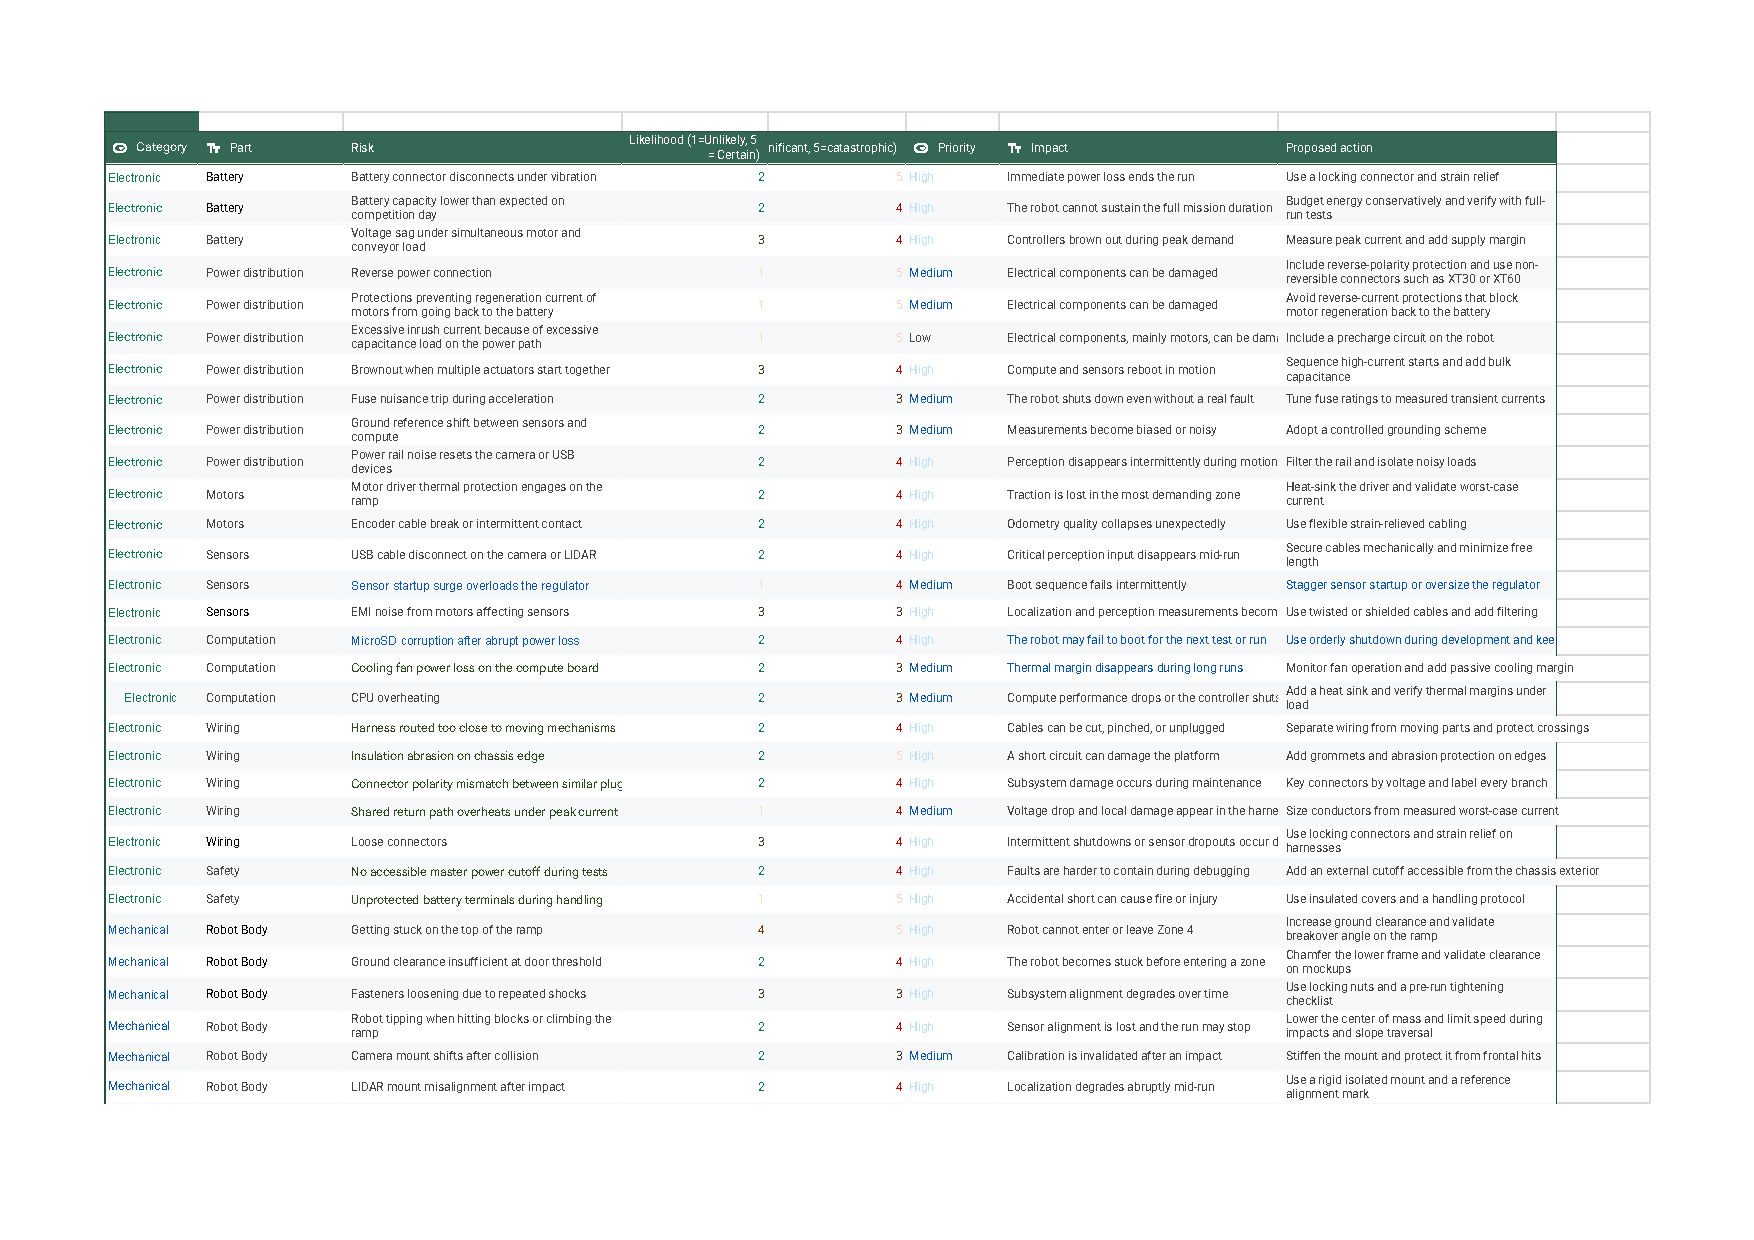
\includepdf[pages=-, pagecommand={\thispagestyle{empty}}, scale=0.92, frame]{documents/Risk Management.pdf}

\subsection*{Appendix C: Code and data}
\addcontentsline{toc}{subsection}{Appendix C: Code and data}
The complete codebase (firmware, ROS~2 workspace, vision, and behaviour tree) is publicly available on the team's GitHub repository: \\
\url{https://github.com/Gwen678/EyeRobot}

\pagebreak

\bibliographystyle{plainnat}
\bibliography{references}

% =====================================================================
% Annexed documents (full milestone deliverables)
% =====================================================================
\cleardoublepage
\phantomsection
\addcontentsline{toc}{section}{Annex: Functional analysis (Milestone~3 document)}
\section*{Annex: Functional analysis (Milestone~3 document)}
The functional analysis document submitted at Milestone~3 is reproduced in full below, including the detailed development schedule and the bill of materials.
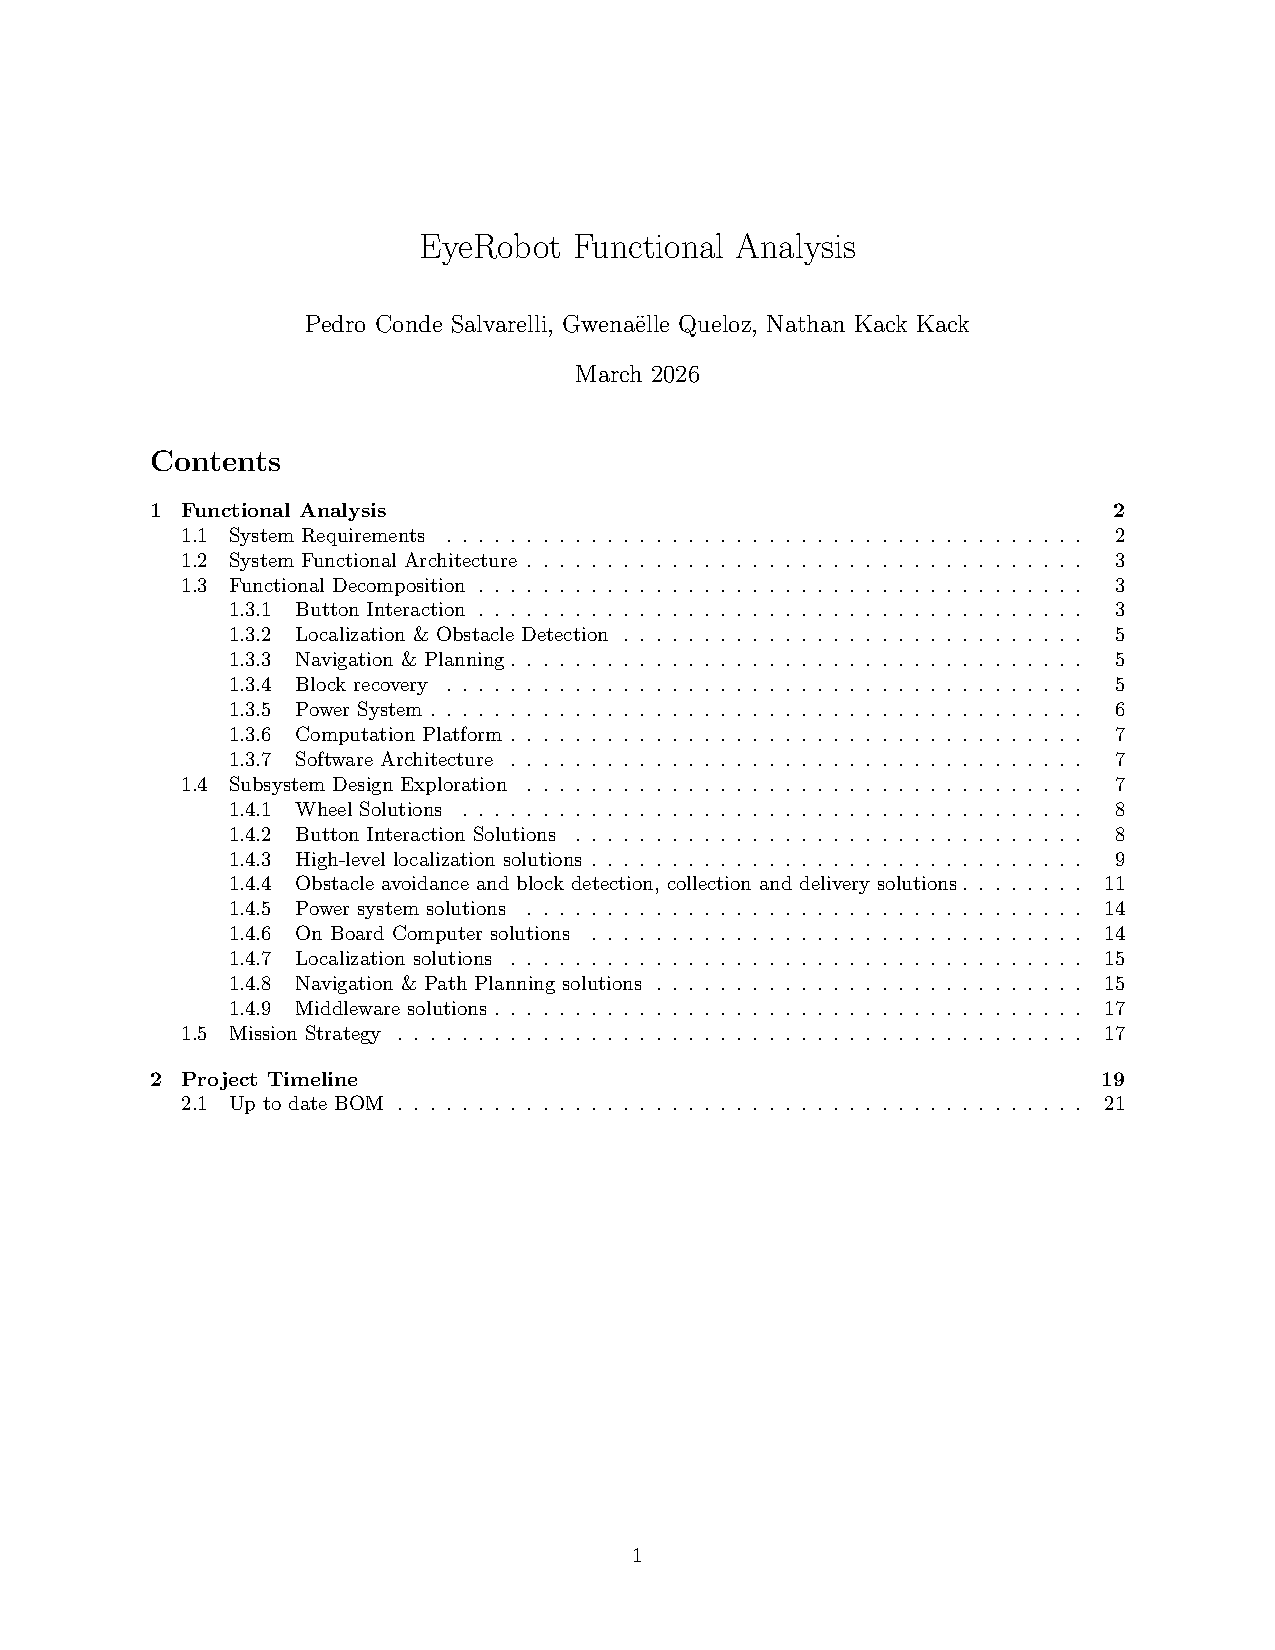
\includepdf[pages=-, pagecommand={\thispagestyle{empty}}]{documents/Functional_Analysis_EyeRobot.pdf}

\end{document}